\documentclass{article}


% if you need to pass options to natbib, use, e.g.:
%     \PassOptionsToPackage{numbers, compress}{natbib}
% before loading neurips_2025


% ready for submission
%\usepackage{neurips_2025}


% to compile a preprint version, e.g., for submission to arXiv, add add the
% [preprint] option:
     \usepackage[preprint,nonatbib]{neurips_2025}


% to compile a camera-ready version, add the [final] option, e.g.:
%     \usepackage[final]{neurips_2025}


% to avoid loading the natbib package, add option nonatbib:
%    \usepackage[nonatbib]{neurips_2025}


\usepackage[utf8]{inputenc} % allow utf-8 input
\usepackage[T1]{fontenc}    % use 8-bit T1 fonts
\usepackage{hyperref}       % hyperlinks
\usepackage{url}            % simple URL typesetting
\usepackage{booktabs}       % professional-quality tables
\usepackage{amsfonts}       % blackboard math symbols
\usepackage{nicefrac}       % compact symbols for 1/2, etc.
\usepackage{microtype}      % microtypography
\usepackage{xcolor}         % colors

\usepackage{array}
\usepackage{lipsum} 
\usepackage{graphicx}
\usepackage{enumitem}
\usepackage{multirow}
\usepackage{multicol}
\usepackage{subcaption}
\usepackage{wrapfig}

\usepackage{enumitem}
\usepackage{mathtools}
\usepackage{ragged2e}
\usepackage{xpatch}
\usepackage{graphicx}
\usepackage{soul}
\usepackage[normalem]{ulem}
\usepackage{pifont}
\usepackage{algorithm}
%\usepackage{algorithmic}
\usepackage{algorithmicx}
\usepackage{algpseudocode}

\usepackage{amsmath}
\usepackage{colortbl}

\usepackage{wrapfig}
\usepackage{adjustbox}

\newcommand{\methodname}{dKV-Cache}
\newcommand{\dmethodname}{dKV-Cache-Decode}
\newcommand{\mmethodname}{dKV-Cache-Greedy}
\newcommand{\pmethodname}{dKV-Cache-Prefill}
\newcommand{\pdmethodname}{dKV-Cache-PD}



\definecolor{Gray}{gray}{0.85}
\definecolor{LightCyan}{rgb}{0.88,0.92,0.92}
\definecolor{bgblue}{RGB}{237, 242, 255}
%\definecolor{bgblue}{RGB}{224,238,255}   % light ‑ for background
\definecolor{fontblue}{RGB}{  0, 70,160} % dark  ‑ for text


\newcommand{\shadowtext}[2][yellow!30]{%
  \begingroup
  \setlength{\fboxsep}{0pt}
  \colorbox{#1}{#2}
  \endgroup
}

\newcommand{\red}[1]{{\color{red}{TODO: #1}}}
\newcommand{\speedtext}[1]{{\small \color{fontblue}{#1}}}
\newcommand{\bx}{\mathbf{x}}
\newcommand{\bh}{\mathbf{h}}
\newcommand{\bq}{\mathbf{Q}}
\newcommand{\bk}{\mathbf{K}}
\newcommand{\bv}{\mathbf{V}}

\newcounter{mycounter} % create a new counter, called 'mycounter'
\newcommand\showmycounter{\stepcounter{mycounter}\themycounter}
\usepackage{tcolorbox}
\newcommand{\findingbox}[1]{
    \stepcounter{mycounter} % Increment counter
    \begin{tcolorbox}[colframe=black,
                      arc=1pt,
                      boxsep=-2pt,
                      ]
        \noindent{\textbf{\textit{Finding \themycounter.}}} #1
    \end{tcolorbox}
}


\title{dKV-Cache: The Cache for Diffusion \\Language Models}


% The \author macro works with any number of authors. There are two commands
% used to separate the names and addresses of multiple authors: \And and \AND.
%
% Using \And between authors leaves it to LaTeX to determine where to break the
% lines. Using \AND forces a line break at that point. So, if LaTeX puts 3 of 4
% authors names on the first line, and the last on the second line, try using
% \AND instead of \And before the third author name.

\author{
\bf Xinyin Ma \quad Runpeng Yu\quad Gongfan Fang\quad Xinchao Wang\thanks{Corresponding author}\\
{National University of Singapore} \\
{\tt\small  maxinyin@u.nus.edu, 
xinchao@nus.edu.sg} \\
% Institution1 address\\
}

\begin{document}


\maketitle


\begin{abstract}

Diffusion Language Models (DLMs) have been seen as a promising competitor for autoregressive language models (ARs). However, diffusion language models have long been constrained by slow inference. A core challenge is that their non‑autoregressive architecture and bidirectional attention preclude the key–value cache that accelerates decoding. We address this bottleneck by proposing a KV-cache-like mechanism, \textbf{d}elayed \textbf{KV-Cache}, for the denoising process of DLMs. Our approach is motivated by the observation that different tokens have distinct representation dynamics throughout the diffusion process. Accordingly, we propose a delayed and conditioned caching strategy for key and value states.
We design two complementary variants to cache key and value step‑by‑step: 
(1) dKV-Cache-Decode, which provides almost lossless acceleration, and even improves performance on long sequences, suggesting that existing DLMs may under‑utilise contextual information during inference. 
(2) dKV-Cache‑Greedy, which has aggressive caching with reduced lifespan, achieving higher speed-ups with quadratic time complexity at the cost of some performance degradation. 
dKV-Cache, in final, achieves from 2-10$\times$ speedup in inference, largely narrowing the gap between ARs and DLMs.  
We evaluate our dKV-Cache on several benchmarks, delivering acceleration across general language understanding, mathematical, and code‑generation benchmarks. Experiments demonstrate that cache can also be used in DLMs, even in a training-free manner from current DLMs. The code is available at https://github.com/horseee/dKV-Cache
%Extensive experiments demonstrate that *KV‑Cache narrows the efficiency gap between diffusion and autoregressive language models, offering a practical pathway to fast, high‑quality text generation without architectural overhaul.
%We further propose a method to largely improve the performance of the model at little extra cost.

\end{abstract}

\section{Introduction}
Diffusion language models (DLMs)~\cite{austin2021structured,hoogeboom2021argmax} have recently emerged as an alternative paradigm for text generation, inspired by the success of diffusion models in continuous domains like images~\cite{esser2024scaling,xie2025sana} and videos~\cite{kong2024hunyuanvideo,videoworldsimulators2024sora}. Unlike autoregressive transformers (ARs) ~\cite{Dubey2024TheL3,Yang2024Qwen25TR,DeepSeekAI2024DeepSeekV3TR} that generate text left-to-right at a time, a diffusion language model produces text by gradually refining a sequence of initially noisy tokens or masked tokens into a coherent output~\cite{ho2020ddpm,li2022diffusion}.
Recent advancements in diffusion-based language models have underscored their versatility across both continuous~\cite{han2022ssd} and discrete formulations~\cite{sahoo2024simple,austin2021structured}. In particular, discrete diffusion models have shown competitive performance in language modeling~\cite{nie2025llada}, attracting growing interest for their potential to achieve faster decoding than traditional ARs while maintaining comparable generation quality.

One notable advantage of diffusion language models is their potential to decode an arbitrary number of tokens in parallel~\cite{xu2025energybased}, whereas ARs require one forward pass per generated token. This parallel decoding paradigm offers the potential for improved wall-clock inference time and higher throughput. However, despite their theoretical efficiency, current DLMs remain substantially slower than ARs in practice. This inefficiency is primarily due to two factors: the incompatibility of DLMs with the KV-Cache mechanism~\cite{lou2023discrete,deschenaux2024promises}, and the large number of network evaluations for denoising~\cite{Feng2025TheoreticalBA}. Specifically, generating a sequence of length $L$ typically entails $L$ denoising steps, each involving a full bidirectional attention pass, leading to a cubic time complexity of $\mathcal{O}(L^3)$. In contrast, AR models utilize KV-Cache to reduce per-step complexity to $\mathcal{O}(L^2)$, achieving much faster inference overall.
%As a result, generating sequences of even moderate length (e.g., 512 tokens) becomes prohibitively slow for DLMs. 

In this paper, we tackle the challenge of integrating the KV-Cache mechanism into diffusion language models and operate without autoregressive or semi-autoregressive structures~\cite{arriola2025block}. We identify two core reasons that prevent the direct usage of KV-Cache in DLMs. 
(1) KV-Cache hinges on the assumption that the key and value states of previously generated tokens remain fixed during subsequent decoding steps. This property is preserved in autoregressive models through the use of a causal attention mask, which restricts each token to attend only to earlier positions~\cite{Dai2019TransformerXLAL}. However, DLMs adopt a bidirectional attention mechanism, similar to non-autoregressive models~\cite{gu2017non}, allowing every token to attend to all others in the sequence and making it nontrivial to reuse previously cached keys and values.
(2) KV-Cache presupposes a fixed and left-to-right sequential decoding, where the position of the next token is deterministic. This assumption enables ARs to compute QKV states selectively only at the current decoding position. However, DLMs break this paradigm by supporting flexible generation orders. At each denoising step, any token position may be selected for update, which is a key advantage of DLMs for tasks involving long-range dependencies and holistic planning~\cite{Ye2025ImplicitSV}. 
%This flexibility precludes the use of targeted QKV computation, thereby undermining the efficiency benefits of KV-Cache.
%In this paper, we focus on the challenge of integrating the KV-Cache mechanism into diffusion language models without relying on the auto-regressive or semi-autoregressive property~\cite{arriola2025block}. 
%We identify two fundamental reasons why the KV-Cache cannot be directly applied to DLMs.
%(1) KV-Cache relies on the assumption that the key and value states of previously decoded tokens remain unchanged throughout subsequent decoding steps. This property is enabled by the causal attention mask used in autoregressive models, which ensures that future tokens do not influence past ones~\cite{Dai2019TransformerXLAL}. In contrast, DLMs employ a bidirectional attention mechanism as in non-autoregressive decoding~\cite{gu2017non}, a defining distinction from AR models, which inherently allows every token to attend to all others in the sequence. Consequently, the representation of a token is no longer static, making it nontrivial to reuse previously computed keys and values.
%Second, the KV-Cache assumes a sequential decoding process in which the position of the next token to be generated is predetermined. This allows for targeted computation of QKV states only at the decoding position. While this assumption naturally aligns with the left-to-right decoding strategy of AR models, it does not hold for DLMs. In DLMs, the generation order is flexible, and any token position may be selected for the next denoising step and is one of the benefits for DLMs for long-term planning~\cite{Ye2025ImplicitSV}. As a result, it becomes infeasible to compute attention selectively for a single token position, further complicating the adoption of KV-Cache.

To solve this problem, we propose the \textbf{d}elayed KV-Cache, \methodname, the KV-Cache for \textbf{d}iffusion language models.
The core design of our proposed dKV-Cache centers on how to enable caching of key and value states across denoising steps in diffusion language models. A key insight motivating this design is that, although DLMs employ bidirectional attention, intuitively incompatible with caching, the representations of key and value are not fundamentally unreusable, but rather require delayed and conditioned reuse.
In particular, we observe that the evolution of key and value states is strongly influenced by whether a token has been decoded. This behavior motivates a delayed caching strategy, wherein only the key and value states of decoded tokens would be cached, delayed from the ARs that caching occurs immediately upon input.
We further propose a one-step delayed caching mechanism, in which the caching of key/value states is postponed by another denoising step. This intentional delay substantially boosts the performance and also reduces memory overhead for KV storage. Besides the delayed caching, we further propose a more aggressive decoding strategy to reduce the computational complexity of diffusion language models from $\mathcal{O}(L^3)$ to $\mathcal{O}(L^2)$ by restricting the caching to a compact subset of tokens: the delayed tokens and the current to-be-decoded tokens, and the window tokens.

Our experiments demonstrate that the proposed method achieves 2–10$\times$ speedup on existing 7B-scale diffusion language models, including LLaDA~\cite{nie2025llada} and Dream~\cite{dream2025}, across a broad range of benchmarks such as general language understanding, code generation, and mathematical problem solving. These efficiency gains come with only minor and often negligible performance degradation, highlighting the practical value of our approach for accelerating DLM inference without training. Furthermore, we demonstrate that \methodname\ is robust across variations in prefill length, output length, and the number of sampling steps.

\paragraph{Contributions.} (1) We propose the first KV-Cache mechanism for diffusion language models by leveraging the evolving dynamics of token representations. We introduce a delay caching strategy compatible with bidirectional attention. (2) We propose two practical variants of our method: \dmethodname, which enables long-term cache reuse, and \mmethodname, which reduces the per-step time complexity for faster decoding. (3) 
Extensive experiments on DLMs demonstrate that our approach achieves 2–10$\times$ inference speedup with minimal or negligible performance loss.


\section{Related Work}
\subsection{Diffusion Language Models}
Diffusion models~\cite{ho2020ddpm,song2019generative} model the data generation as the inversion of a forward-noise process and demonstrated impressive generation quality in image~\cite{peebles2023dit}, video~\cite{videoworldsimulators2024sora}, and audio generation~\cite{Evans2024FastTL}. 
For diffusion models on language generation, ~\cite{hoogeboom2021argmax,austin2021structured} extends DDPM to categorical data and defines the transition matrices for the corruption and denoising. ~\cite{li2022diffusion} introduces the continuous-time diffusion over the continuous word-embedding space, and ~\cite{han2022ssd} closes the quality of generation on par with GPT-2 via a simplex defined over the vocabulary. Besides the diffusion in the continuous space~\cite{wu2023ar,ye2023dinoiser} for discrete distribution, another approach seeks the path in discrete language diffusion models. ~\cite{he2022diffusionbert} training BERT to learn the reverse process of a discrete diffusion process with an absorbing state in D3PM. 
SEDD~\cite{lou2023discrete} introduces score entropy training, a novel loss extending score-matching to discrete data and MDLM~\cite{sahoo2024simple} shows that simple masked discrete diffusion is competitive to all previous kinds of DLMs.
Block diffusion ~\cite{arriola2025block} extends the current non-autogressive~\cite{gu2017non} discrete language diffusion models into a semi-autoregressive one~\cite{han2022ssd,zhao2024pard}, making it feasible to generate sequences of arbitrary length. ~\cite{nie2025llada,gong2024scaling} scaling the masked diffusion language models to billions of parameters, achieving performance comparable to leading autoregressive LLMs.




\subsection{Cache in Generative Models}
Cache~\cite{wilkes2006slave} is a small, fast memory that stores frequently accessed data, reducing the time that the CPU needs to fetch data from slower memory. Cache is first introduced in deep neural networks in transformers~\cite{vaswani2017attention}, where the KV-Cache caches previous tokens' key and value tensors. KV-Cache becomes a fundamental technique in transformers, and several improved techniques are proposed~\cite{ge2024model,liu2023scissorhands,hooper2024kvquant} to reduce the memory consumption of KV-Cache for long-context generation. Besides this, caches are also been explored in diffusion models for image~\cite{ma2023deepcache,wimbauer2023cache}. Those work leverage the temporal similarities between high-level features~\cite{ma2024learning,chen2024delta}, attention map~\cite{yuan2024ditfastattn,liu2024faster} to achieve faster inference of diffusion generation. This also has been explored in 3D generative modeling~\cite{yang2024hash3d} and video generation~\cite{zhao2024real,lv2024fastercache}. However, the cache for diffusion language models is less explored, especially the KV-Cache for diffusion language models. ~\cite{arriola2025block} explores the kv-cache in semi-autoregressive diffusion language models. This requires considering the KV-Cache in training, making twice the forward computation in the training and its form is still constrained in the autoregressive formula. ~\cite{sahoo2024simple} also considers cache, but under a strict condition that no new tokens have been calculated.



\section{Methods}

\subsection{Preliminary}
We primarily focus on continuous-time discrete language models, with particular attention to masked diffusion language models~\cite{sahoo2024simple,nie2025llada}, which have shown strong scalability to billion-parameter scales with high generation quality.

Consider a text sequence with $L$ tokens $\mathbf{x}^{1:L}_0$, sampled from the target distribution $p_{data}(\mathbf{x}_0)$. Each token is represented by a one-hot vector with $V$ categories, where $V$ is the vocabulary size. 
The forward process adds noise in the original sequence $\mathbf{x}_0$, which, in the discrete diffusion models here, takes the form of masking some of the tokens randomly. 
The masking process can be controlled by a transition matrix $\boldsymbol{U}_t$, where each element in this matrix $\left[\boldsymbol{U}_t\right]_{ij}$ represents the probability transition from token $i$ to token $j$ at step $t$~\cite{austin2021structured}. The denoising process is discretized into $T$ steps, and we define the continuous timestep $c(t) = t / T$, where $t \in \{0, 1, \ldots, T\}$. We use \emph{timestep} in the continuous temporal space of the denoising process and \emph{step} in the discrete space. The forward diffusion can be modelled as:
\begin{align*}
    q\left(\boldsymbol{x}_{c(t)} \mid \boldsymbol{x}_0\right)=\operatorname{Cat}\left(\boldsymbol{x}_{c(t)} ; \boldsymbol{p}=\boldsymbol{x}_0 \overline{\boldsymbol{U}}_{t}\right), \quad \text { where } \quad \overline{\boldsymbol{U}}_{t}=\prod_{i=1}^t\boldsymbol{U}_i
\end{align*}
Then we can get the corrupted $\mathbf{x}_0$. The absorbing form for the transition matrix is used here, where each token either remains the same or transfers to the special [MASK] token at the probability of $\beta_t$. The cumulated transition matrix $\overline{\boldsymbol{U}}_t$, as defined in the masked diffusion models, can be formulated as:
\begin{align*}
    \left[\overline{\boldsymbol{U}}_t\right]_{ij}=\left\{\begin{array}{lll}
1 & \text { if } \quad i = j = \text{[MASK]} \\
\bar{\alpha}_t & \text { if } \quad i=j \neq \text{[MASK]} \\
1 - \bar\alpha_t & \text { if } \quad j=m, i \neq \text{[MASK]} 
\end{array}\right. \quad \text { with } \bar\alpha_t = \prod_{i=1}^t\left(1 -\beta_i\right)
\end{align*}
where $\bar\alpha_t$ linearly decrease to 0 as $t$ approaches T.
The reverse process is learned by the models $\theta$, where $p_{\theta}(\mathbf{x}_{c(t-1)}|\mathbf{x}_{c(t)})$ is learned to approximate $q(\mathbf{x}_{c(t-1)}|\mathbf{x}_{c(t)}, \mathbf{x}_0)$. In $p_{\theta}(\mathbf{x}_{c(t-1)}|\mathbf{x}_{c(t)})$, the neural network with parameters $\theta$ is optimized to predict the clean tokens $\mathbf{x}_0$ given $\mathbf{x}_{c(t)}$. 

\paragraph{Sampling Process of DLMs.} Given the noisy sequence $x_1^{1:L}$, which is consisted only with the masked token. Each timestep, the denoising model $p_{\theta}(\mathbf{x}_{c(t-1)}|\mathbf{x}_{c(t)})$ would be called, with $x_0$ predict first and then remasking the rest by $q(\mathbf{x}_{c(t-1)}|\mathbf{x}_0, \mathbf{x}_{c(t)})$. The unmasked tokens would remain unchanged during the later denoising process. Several strategies are used in the remasking stage, e.g., random remasking~\cite{austin2021structured}, keeping the most confident ones ~\cite{chang2022maskgit} or by selecting the topk positions with the largest margin between the two most probable values~\cite{kim2025train}.

\begin{figure}[t]
    \centering
    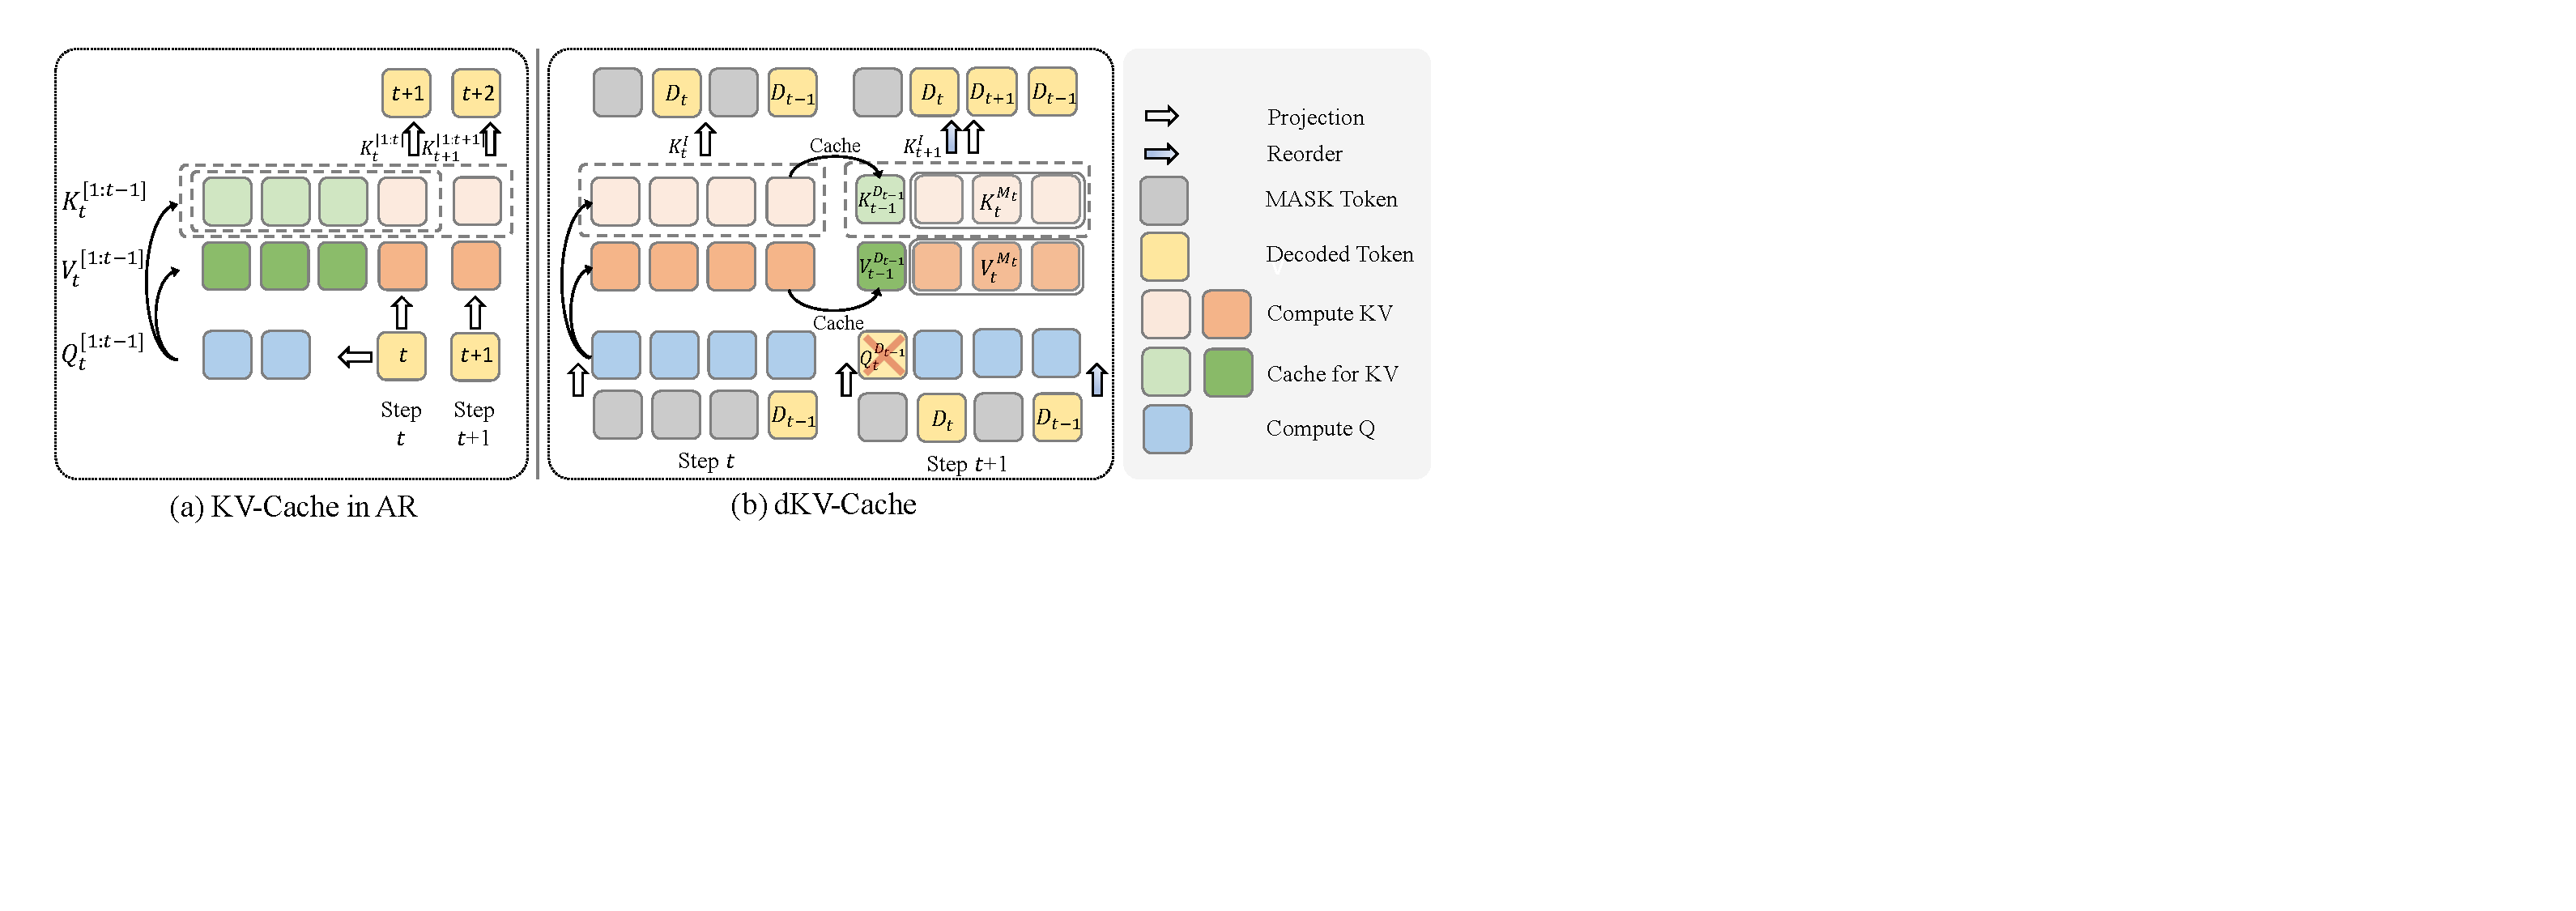
\includegraphics[width=\linewidth]{figure/main_v8.pdf}
    \caption{Illustration of \methodname. At step $t$, no prior cache would be activated though the token $D_{t-1}$ has been decoded. $\bk$ and $\bv$ are delayed to the next step to be reordered and reused.}
    \label{fig:main_figure}
\end{figure}

\paragraph{Formulation of KV-Cache.}
Since diffusion language models still use the transformer architecture (with or without GQA~\cite{ainslie2023gqa} would not affect our method), we simply grab the formulation of KV-Cache in ARs first. In a transformer decoder, each layer would project the current hidden states $\bh_t$ into a query-key-value triplet $(\bq_t, \bk_t, \bv_t)$ via learned projection $\mathbf{W_Q}, \mathbf{W_K}$ and $\mathbf{W_V}$. At step $t$, only the hidden states of the $t$-th tokens $\bh_t^{[t]}$ would be calculated. The recursive KV‑Cache update is appending the new key–value pair to the running buffered KV-Cache:
\begin{align}
    \mathbf{z}_t=\operatorname{softmax}\left(\frac{\mathbf{Q}_t^{[t]}\left(\mathbf{K}_t^{[1: t]}\right)^{\top}}{\sqrt{d_k}}\right) \mathbf{V}^{[1: t]} \quad \text{ with } \left\{\begin{array}{l} \mathbf{K}_t^{[1: t]}=\operatorname{concat}\left(\mathbf{K}_{t-1}^{[1: t-1]}, \mathbf{K}_t^{[t]}\right) \\ \mathbf{V}_t^{[1: t]}=\operatorname{concat}\left(\mathbf{V}_{t-1}^{[1: t-1]}, \mathbf{V}_t^{[t]}\right)\end{array} \right. \label{eq:kv-cache}
\end{align}
where $\mathbf{z}_t$ is the output of the attention head at step $t$ and the dot products are scaled down by $\sqrt{d_k}$. 

\subsection{Why KV-Cache Cannot be Used in DLMs?}
%We want to explore how to make the KV-Cache work in diffusion language models, and in the following section, we gradually switch a KV-Cache in the auto-regressive models into the KV-Cache in the diffusion language models by analysing and then adding key designs into the KV-Cache.
The effectiveness of KV-Cache can be attributed to the reuse of previously computed K and V states, and the targeted computation only for the current decoding token. We conclude that standard KV-Cache is fundamentally incompatible with diffusion language models for two reasons:
\begin{itemize}
    \item \textbf{Timestep-variant key and value states.} In the autoregressive setting, every time step shares a single, causally growing set of key and value tensors. $\mathbf{K}_m^{[1: t-1]}$ and $\mathbf{V}_m^{[1: t-1]}$ are the same at each step $m$ from $t-1$ and later with the help of causal attention mask. By contrast, DLMs employ a bidirectional attention mask; consequently, the key and value representations that each token can attend to at timestep $m$,  $\mathbf K_m^{[1:t-1]}$ and $\mathbf V_m^{[1:t-1]}$, differ from those at timestep $n$. Put differently, $\mathbf K_m^{[1:t-1]} \neq \mathbf K_n^{[1:t-1]}$ and $\mathbf V_m^{[1:t-1]} \neq \mathbf V_n^{[1:t-1]}$ if $n\neq m$. The bidirectional attention introduced by diffusion language models therefore breaks the global reuse assumption that supports conventional KV‑Cache.
    \item \textbf{Non‑sequential decoding order.} Generation in DLMs does not follow a strictly left-to-right order. Instead, the model dynamically fills masked positions based on probabilities computed at each denoising step. As a result, the positions of decoded tokens are only revealed after the model forward pass, and the subsequent update may target any position in the sequence, rather than progressing sequentially. This uncertainty prevents us from pre-determining which token $i$ will require the computation of its hidden states $\bh^{[i]}$ and its $\mathbf{Q}^{[i]}$, $\mathbf{K}^{[i]}$ and $\mathbf{V}^{[i]}$.
\end{itemize}
%For the auto-regressive models, $\mathbf{K}_i^{[1: t-1]}$ and $\mathbf{V}_i^{[1: t-1]}$ are the same at each step $i$ from $t-1$ and later with the help of causal attention mask, making the computational results reusable. Besides, since the sequential order of decoding that each time, the position of the new token would always be the next token for the current sequence. Thus each time, the query, key, values for the next token would be calculated. Together with the previously-cached results, the generation can be largely accelerated, with $\mathcal{O}(L^2)$ as the time complexity.


\paragraph{Representation Dynamics for tokens in Diffusion Sampling}
We investigate in DLMs whether $\bk$ and $\bv$ can be reused. We focus on the dynamics of $\bk$ and $\bv$ for each token, and the results are shown in Figure \ref{fig:token_evolve}.
\begin{figure}[t]
    \centering
    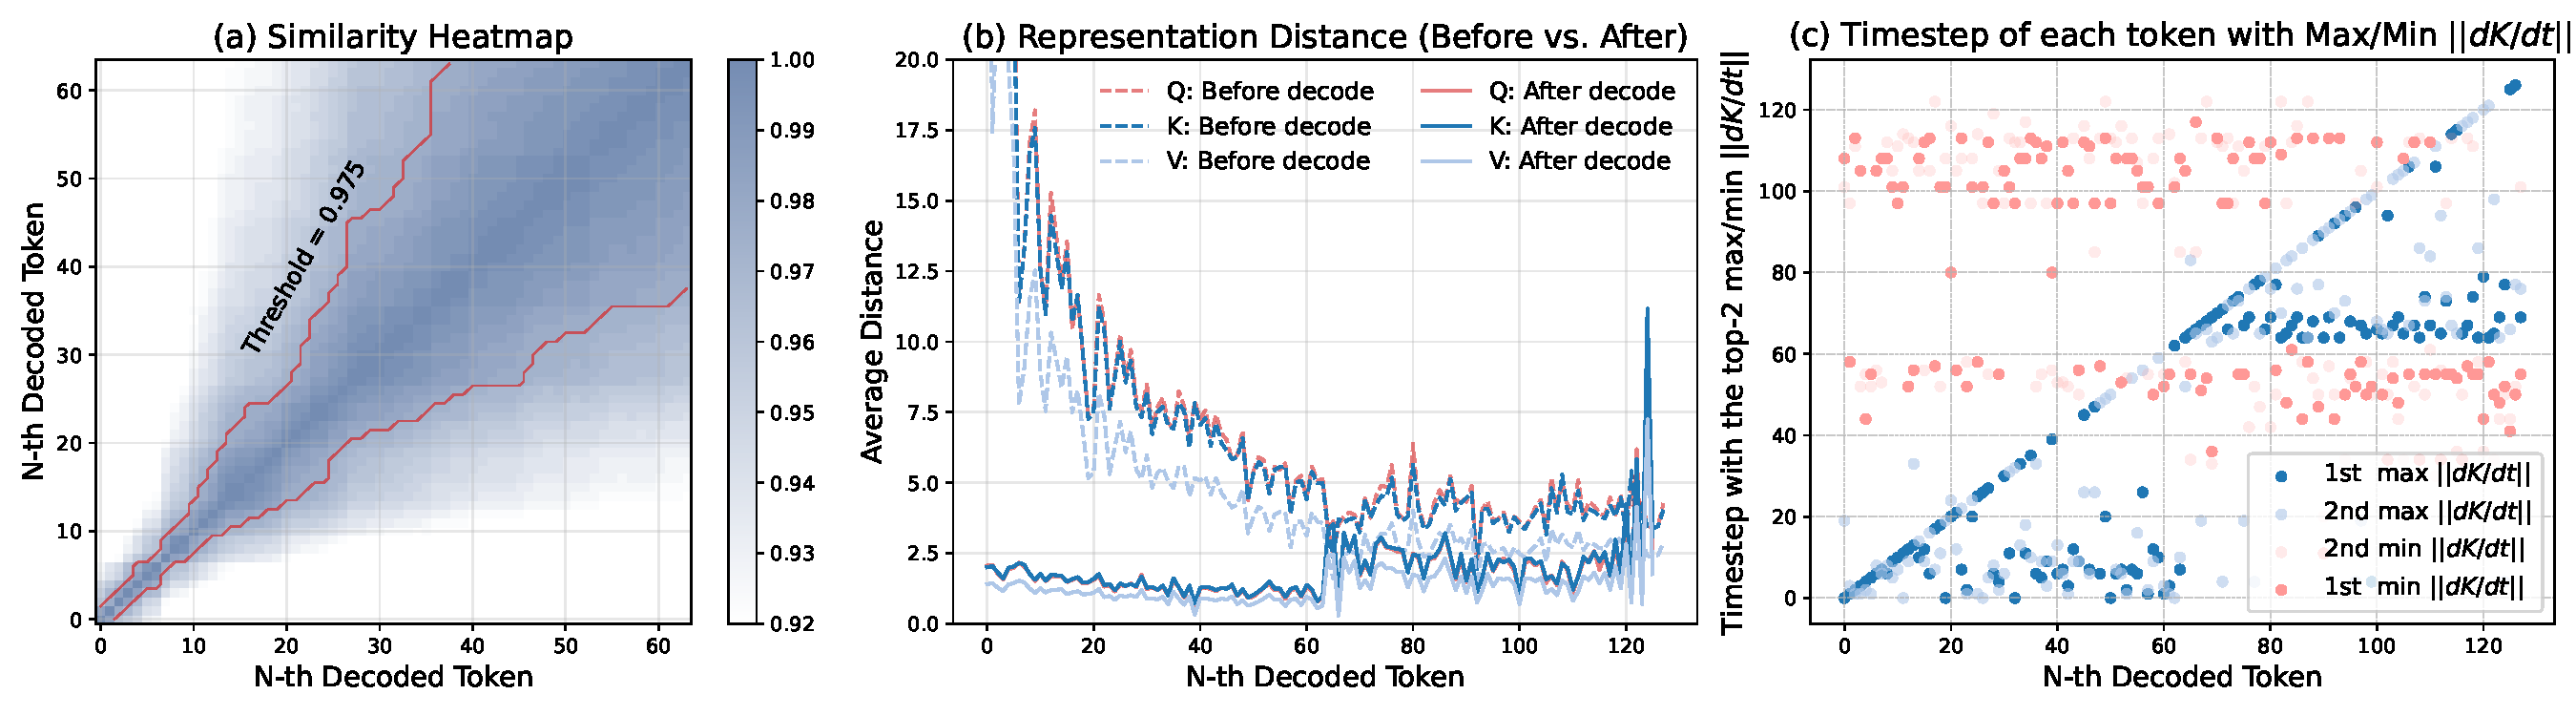
\includegraphics[width=1.\linewidth]{figure/token_dynamics_v3.pdf}
    \caption{(a) We present a heatmap illustrating the pairwise similarities among the key states across different timesteps. Here we use LLaDA with $L=128$, $T=128$ and the block size is set to 64. We then compute the Euclidean distance between consecutive steps $t$ and $t+1$ to analyze the dynamics of intermediate representations. (b) We report the average distance measured before and after the decoding of each token. (c) We highlight the top-2 steps exhibiting the largest and smallest changes in the key and value states for each token in their decoded order. }
    \vspace{-5mm}
    \label{fig:token_evolve}
\end{figure}
%This approach relies on a strong assumption that the cached key states from the previous step, $\mathbf{K}_{t-1}^{\mathcal I}$, can be reused as a valid approximation for $\mathbf{K}_{t}^{\mathcal I}$ in the current step. This assumption directly corresponds to Issue 2 discussed earlier. However, in diffusion language models, the input representation is inherently updated at each decoding step, which inevitably leads to discrepancies in intermediate representations across successive timesteps. This temporal inconsistency is a primary factor contributing to the observed performance degradation, even after the modifications described above. We conduct a more detailed analysis of this issue in Figure \ref{}. 
Interestingly, we observe several noteworthy patterns in the dynamics of QKV states:
(1) Despite step-to-step differences, the key and value embeddings, $\bk$ and $\bv$, exhibit consistently high similarity across timesteps, as shown in Figure \ref{fig:token_evolve}(a).
(2) Once a token is decoded, its representation becomes relatively stable in subsequent steps, whereas the representations of still-masked tokens continue to fluctuate significantly. This phenomenon is evident in Figure \ref{fig:token_evolve}(b), where QKV fluctuations are more pronounced prior to decoding than thereafter.
(3) The most substantial changes in $\bk$ and $\bv$ occur at the decoding step of each token and then in the early stages of the denoising process. This is reflected by prominent changes along the diagonal in Figure \ref{fig:token_evolve}(c), corresponding to the $i$-th decoding step which decodes the $i$-th token. 

These observations provide key insights into the temporal structure of discrete diffusion models and motivate the design of our KV-Cache mechanism for diffusion language modeling.

%Interestingly, we observe several notable phenomena in the dynamics of intermediate states: 
%(1) Though different, the similarities are still high for $\bk$ and $\bv$ between different steps in Figure \ref{fig:token_evolve}(c) 
%(2) Once a token is decoded, its representation becomes relatively stable in subsequent steps, whereas the representations of still-masked tokens continue to fluctuate much larger. In Figure \ref{fig:token_evolve}(b), where the fluctuations of QKV representations are much obvious before the tokens are generated, but remain relatively stable after it is decoded.
%(3) The most change happens at the step is decoded, then the beginning of the denoising process. In figure \ref{fig:token_evolve}(c), a lot of changes happens at the diagonal part, which is the $i$ step for the $i$-th decoded token. Besides, the larger $\left\| \frac{dK}{dt}\right\|$ is observed before the token is decoded (the lower triangular part of the figure), while the representations become stable at the end of the decoding for a block of for the whole diffusion sequence.
%Those behaviour of discrete diffusion models motivates us to develop the below KV-Cache for diffusion-based language models.

\subsection{Delayed KV-Cache for Masked Diffusion Language Models}
We first present a more general non‑sequential KV‑Cache formulation that replaces the contiguous slice $\text{K}^{[1{:}t-1]}$ used in Eq.\ref{eq:kv-cache} with an arbitrary-order index set $\mathcal S_t\subseteq \mathcal I=\{1,\dots,L\}$ and the next token position from the fixed $t$ to $D_t$. The cached keys and values gathered from previous steps are now $\mathbf{K}_t^{\mathcal{S}_t}$, which retrieves cached states at the positions specified by indexes in $\mathcal S_t$:
\begin{equation}
\small
    \mathbf{z}_t=\operatorname{softmax}\left(\frac{\mathbf{Q}_t^{D_t}\left(\mathbf{K}_t^{\mathcal{S}_t \cup\{D_t\}}\right)^{\top}}{\sqrt{d_k}}\right) \mathbf{V}_t^{\mathcal{S}_t \cup\{D_t\}} \text{ with } \left\{\begin{array}{l} \mathbf{K}_t^{\mathcal{S}_t \cup\{t\}}=\operatorname{concat\_reorder}\left(\mathbf{K}_{t-1}^{\mathcal{S}_t}, \mathbf{K}_t^{D_t}\right) \\ \mathbf{V}_t^{\mathcal{S}_t \cup\{t\}}=\operatorname{concat\_reorder}\left(\mathbf{V}_{t-1}^{\mathcal{S}_t}, \mathbf{V}_t^{D_t}\right) \end{array}\right. \label{eq:set_kv}
\end{equation}
where $D_t$ is the denoised token at step $t$. If we use random sampling for diffusion, then before any inference, we can know the decoding order of the sequence. We here use the notation of $D_t$, and later would not depend on knowing the decoding order. 
The operator $\operatorname{concat\_reorder}$ is proposed to enhance the efficiency of the indexing and gathering of K and V here. 
We explain in the appendix about this operator and how it works with ROPE~\cite{su2024roformer} and how it accelerates.

We first extend the formulation in Eq.\ref{eq:set_kv} by generalizing the query input $\bq_t^{D_t}$ from the single-token decoding to the multiple and arbitrary token decoding. Specifically, at decoding step $t$, we construct a dynamic set $\mathcal{M}_t$, where $\mathcal{M}_t$ denotes the subset of tokens that are not yet finalized during generation. 
And with the $\mathbf{h}_t^{\mathcal{M}_t}$ calcuated, we also can get the corresponding $\mathbf{Q}_t^{\mathcal{M}_t}$, $\mathbf{K}_t^{\mathcal{M}_t}$ and $\mathbf{V}_t^{\mathcal{M}_t}$. We delay the caching of each token, not the time it is appended in the input, but rather on the step it is decoded:
\begin{align}
    \operatorname{concat\_reorder}\left(\right.\underbrace{\mathbf{K}_{t-1}^{\mathcal{S}_t}}_{\text{Cache from } t-1}, \underbrace{\mathbf{K}_t^{D_t}}_{\text{Calcualte at } t}\left.\right) \Rightarrow \operatorname{concat\_reorder}\left(\right.\underbrace{\mathbf{K}_{t-1}^{\mathcal{I}\setminus\mathcal{M}_t}}_{\text{Cache from } t-1}, \underbrace{\mathbf{K}_t^{\mathcal{M}_t}}_{\text{Calculate at } t}\left.\right) 
\end{align}
where $\mathcal{I}$ denotes the set of all tokens involved in the denoising process. This design reflects our core observation in the previous section: only the decoded tokens are eligible for caching, while the remaining masked tokens must be re-encoded at each step. Besides, this method solves the problem that we need to predefine or predict the denoising order, as $\mathcal{M}_t$ is explicitly known at each step.
%Thus, the caching is delayed after the tokens have been decoded.  The attention computation is thus reformulated as:
%\begin{align}
%\mathbf{z}_t=\operatorname{softmax}\left(\frac{\mathbf{Q}_t^{\mathcal{M}_t}\left(\mathbf{K}_t^{\mathcal{I}}\right)^{\top}}{\sqrt{d_k}}\right) \mathbf{V}_t^{\mathcal{I}}, \quad \text{ with } \left\{\begin{array}{l} \mathbf{K}_t^{\mathcal{I} } =\operatorname{concat\_reorder}\left(\mathbf{K}_{t-1}^{\mathcal{I}\setminus \mathcal{M}_t}, \mathbf{K}_t^{\mathcal{M}_t}\right) \\ \mathbf{V}_t^{\mathcal{I}}=\operatorname{concat\_reorder}\left(\mathbf{V}_{t-1}^{\mathcal{I}\setminus\mathcal{M}_t}, \mathbf{V}_t^{\mathcal{M}_t}\right) \end{array}\right.
%\end{align}
Cached keys and values corresponding to $\mathcal{I}\setminus \mathcal{M}_t$ are reused across steps, while non-finalized positions are recomputed at each step to ensure correctness under bidirectional attention masking.

\paragraph{One-step Delayed Caching.} As our analysis in Figure \ref{fig:token_evolve}(c), the most significant change in $\bk$ and $\bv$ occurs exactly at the step where a token transitions from [MASK] to its decoded form. Currently, $\mathbf{K}_t^{D_t}$ would be used for caching, as it is no longer in the masked set $\mathcal{M}_t$. However, $\mathbf{K}_t^{D_t}$ can differ substantially from $\mathbf{K}_{t+1}^{D_t}$, and prematurely reusing it lead to severe performance degradation. To address this, we introduce one-step delayed caching. At timestep $t$, we use the masking state from the previous step, $\mathcal{M}_{t-1}$, to determine which tokens are cacheable. The method, named \dmethodname, is finally formalized as:
\begin{align}
    \mathbf{z}_t=\operatorname{softmax}\left(\frac{\mathbf{Q}_t^{\mathcal{M}_{t-1}}\left(\mathbf{K}_t^{\mathcal{I}   }\right)^{\top}}{\sqrt{d_k}}\right) \mathbf{V}_t^{\mathcal{I}} 
    \text{ with } \left\{\begin{array}{l} \mathbf{K}_t^{\mathcal{I}}=\operatorname{concat\_reorder}\left(\mathbf{K}_{t-1}^{\mathcal{I}\setminus\mathcal{M}_{t-1}}, \mathbf{K}_{t}^{\mathcal{M}_{t-1}}\right) \\ \mathbf{V}_t^{\mathcal{I}}=\operatorname{concat\_reorder}\left(\mathbf{V}_{t-1}^{\mathcal{I}\setminus\mathcal{M}_{t-1}}, \mathbf{V}_{t}^{\mathcal{M}_{t-1}}\right) \end{array}\right. 
    \label{eq:kv_decode}
\end{align}
While this slightly reduces efficiency, we find it to be critical for maintaining accuracy and stability in the proposed dKV-Cache mechanism for diffusion language models. 

%the biggest change of representation happens exactly at the step when the token changes from [MASK] to the unmasked one. Assume that in step $t$, the decoded token is $d_t$. $\mathbf{K}_{t}^{[d_t]}$ would be cached and reused in the next step since it's not in $\mathcal{M}_t$. However, $\mathbf{K}_{t}^{[d_t]}$ would be largely different from $\mathbf{K}_{t+1}^{[d_t]}$ and thus, reuse it would cause serve performance drop. We delay one more step for the decoded tokens to be cached, which means that at timestep $t$, we use $\mathcal{M}_{t-1}$ instead of $\mathcal{M}_t$. It would hurt some efficiency, but we found is the key to the success of dKV-Cache in DLMs.

\paragraph{Cache Refreshing Mechanism.} While it is possible to apply caching after each token is decoded and reuse it throughout the denoising process, in practice, when the sequence is sufficiently long, occasionally recomputing the cache incurs small computational overhead. To maintain consistency and improve correctness during decoding, we add a cache refreshing mechanism. Every N steps, the stored cache would be discarded and refreshed. The calculation would revert back to the normal calculation, resulting in an empty set $\emptyset$ to replace $\mathcal{M}_{t-1}$ for this refresh step in Eq.\ref{eq:kv_decode}. 

\paragraph{\pmethodname\ and \pdmethodname.} The set $\mathcal{M}_{t-1}$ can be further divided into two subsets: decoded tokens and always-decoded tokens, i.e., prefill tokens. Our experiments show that prefill tokens primarily attend to each other, indicating limited influence from later tokens. Based on this, we adopt a special strategy, \pmethodname, that caches prefill tokens without refreshing. This design aligns with the disaggregation of prefill and decoding phases~\cite{Zhong2024DistServeDP} for serving DLMs. Building on this, we have another variant, \pdmethodname, which intermittently refreshes only the newly decoded tokens, while keeping the key and values of prefill tokens without any recomputation.


\subsection{dKV-Cache-Greedy: Greedy Formulation of dKV-Cache}

However, the above method still incurs $\mathcal{O}(L^3)$ complexity, which is less efficient than the $\mathcal{O}(L^2)$ complexity of ARs. This is primarily because $\mathcal{M}_t$ initially consists of the entire sequence with $L$ tokens and only narrows to a single token at the end. To improve efficiency, it is essential to decouple $|\mathcal{M}_t|$ for each step from the sequence length $L$.

Instead of the minimally refreshed caches proposed above, we adopt a more relaxed cache mechanism to refresh more so as to mitigate the performance degradation caused by stale $\bk$ and $\bv$. Building on our earlier observation that token representations undergo significant changes at their decoding step, we define $\mathcal{M}_t$ to include only three components: the token at the current step $D_t$, the token from the previous step $D(t-1)$ (motivated by one-step delayed caching), and a local window $\mathcal{W}(t)$. For this local window, we extend it to include the token itself and its neighboring tokens within a fixed-size window $\mathcal{W}_t=\left\{x_i \left\lvert\, i \in\left[ D_t-\left\lceil\frac{w}{2}\right\rceil, D_t+\left\lfloor\frac{w}{2}\right\rfloor\right]\right.\right\}$, where $w$ is the window size. We evaluated local windows centered at both $D_t$ and $D_{t-1}$, and found that the latter yields better performance. Since the window size $|\mathcal{W}_t|$ is fixed (set to at most 6 in our experiments), this strategy introduces additional computation but retains an overall time complexity of $\mathcal{O}(L^2)$.


\begin{table}[t!]
    \centering
    \caption{Benchmark results on LLaDA-8B-Instruct. We use zero-shot evaluation here. Detailed configuration is listed in the Appendix. We set the cache refresh step for \dmethodname\ to be 8 and \mmethodname\ to be 2. The window size of \mmethodname\ is listed in the bracket.}
    \resizebox{1.0\linewidth}{!}{
    \begin{tabular}{c||cc|cc||cc|c}
        \toprule
        & Base & Few-Steps &  \mmethodname & \mmethodname & Base & Half-Steps & \dmethodname \\
        Remasking & \small (random) & \small (random) & \small (random) & w/ Window \small (random) & \small (confidence) & \small (confidence)  & \small (confidence) \\
        \midrule
        MMLU     & 51.79 & 43.19 & 45.77 & 47.70 (4) & 51.11 & 51.11 & 51.00 \\ %51.18  &  50.89 & 51.06 \\ % 32, 32, 16
        & \speedtext{30.20} & \speedtext{47.49 \shadowtext{(1.67$\times$)}} & \speedtext{50.56 \shadowtext{(1.57$\times$)}} & \speedtext{45.72 \shadowtext{(1.51$\times$)}} &  \speedtext{28.27} &  \speedtext{55.80 \shadowtext{(1.97$\times$)}} & \speedtext{66.52 \shadowtext{(2.35$\times$)}} \\
        \midrule
        GSM8K   & 72.25 &  65.58 & 67.93 &  68.23 (4) & 77.56  &  77.91 & 78.85 \\
        & \speedtext{15.16} & \speedtext{24.08 \shadowtext{(1.59$\times$)}} & \speedtext{25.47 \shadowtext{(1.68$\times$)}} & \speedtext{24.76 \shadowtext{(1.63$\times$)}} & \speedtext{14.31} & \speedtext{28.71 \shadowtext{(2.00$\times$)}} & \speedtext{27.50 \shadowtext{(1.92$\times$)}} \\
         \arrayrulecolor{gray!50}\cmidrule(lr){2-8} 
         \arrayrulecolor{black}   
        %GSM8K   & 68.16 & 54.89 & 58.76 &  60.58 & 77.91 & 73.31 & 76.95 \\
        % \\
         %\arrayrulecolor{gray!50}\cmidrule(lr){2-8} 
         %\arrayrulecolor{black}   
        Math500  & 27.4 & 21.8 & 26.0 & 27.0 (4) & 36.6  & 34.2 & 36.8 \\
        & \speedtext{12.00} & \speedtext{19.36 \shadowtext{(1.61$\times$)}} & \speedtext{20.34 \shadowtext{(1.70$\times$)}} & \speedtext{19.86 \shadowtext{(1.66$\times$)}} & \speedtext{11.53} & \speedtext{23.10 \shadowtext{(2.00$\times$)}} & \speedtext{24.46 \shadowtext{(2.12$\times$)}}\\
        \arrayrulecolor{gray!50}\cmidrule(lr){2-8} 
         \arrayrulecolor{black}   
        GPQA      & 27.46 & 24.78 & 26.79 & 28.35 (4) & 30.80 & 27.68 & 28.13 \\
        & \speedtext{11.40} & \speedtext{18.59 \shadowtext{(1.63$\times$)}} & \speedtext{19.27 \shadowtext{(1.69$\times$)}} & \speedtext{18.26 \shadowtext{(1.60$\times$)}} & \speedtext{11.86} & \speedtext{23.88 \shadowtext{(2.01$\times$)}} & \speedtext{28.73 \shadowtext{(2.42$\times$)}}\\
        
        \midrule
        HumanEval   & 19.88 & 15.61 & 15.13 & 15.37 (4) & 39.63 & 33.54 & 46.34 \\
        & \speedtext{7.50} & \speedtext{12.50 \shadowtext{(1.67$\times$)}} & \speedtext{12.31 \shadowtext{(1.64$\times$)}} & \speedtext{12.13 \shadowtext{(1.62$\times$)}} & \speedtext{7.08} & \speedtext{14.18 \shadowtext{(2.00$\times$)}} & \speedtext{13.76 \shadowtext{(1.83$\times$)}} \\
        \arrayrulecolor{gray!50}\cmidrule(lr){2-8} 
         \arrayrulecolor{black}  
        MBPP & 21.4 & 15.6 & 17.8 & 20.4 (2) & 40.4 & 33.8 & 40.4\\
        & \speedtext{7.51} &  \speedtext{12.97 \shadowtext{(1.73$\times$)}} & \speedtext{12.55 \shadowtext{(1.67$\times$)}} & \speedtext{12.44 \shadowtext{(1.66$\times$)}} & \speedtext{7.50} & \speedtext{15.01 \shadowtext{(2.00$\times$)}} & \speedtext{13.93 \shadowtext{(1.86$\times$)}}\\
        \bottomrule
    \end{tabular}
    }
    \label{tab:table_llada}
\end{table}

\begin{table}[t!]
    \centering
    \caption{Benchmark results on Dream-Base-7B. We use the few-shot ICL here and the configuration is in Appendix. We set the cache refresh interval for \dmethodname\ and \pdmethodname\ to 4.}
    \resizebox{1.0\linewidth}{!}{
    \begin{tabular}{cc|cc|ccc}
        \toprule
        & & Dream-7B & Half-Steps & \dmethodname & \pmethodname & \pdmethodname  \\
        \midrule 
        % GSM8K
        \multirow{4}{*}{\shortstack[c]{GSM8K \\ (8-shot) \\ L = 256}} & \multirow{2}{*}{T = 256} & 76.88 & 68.08 & 76.57 & 75.66 & 74.07 \\
        & & \speedtext{15.1 \shadowtext{(1.00$\times$)}} & \speedtext{30.3 \shadowtext{(2.00$\times$)}} & \speedtext{31.6 \shadowtext{(2.09$\times$)}} & \speedtext{53.6 \shadowtext{(3.55$\times$)}} & \speedtext{50.2 \shadowtext{(3.32$\times$)}}\\
         \arrayrulecolor{gray!50}\cmidrule(lr){2-7} 
         \arrayrulecolor{black}   
        & \multirow{2}{*}{T = 128} & 68.81 & 46.63 & 65.35 & 65.96 & 63.31\\
        & \speedtext{} & \speedtext{30.3 \shadowtext{(2.01$\times$)}} & \speedtext{60.5 \shadowtext{(4.01$\times$)}} & \speedtext{62.31 \shadowtext{($4.13\times$)}} & \speedtext{107.4 \shadowtext{($7.11\times$)}} & \speedtext{99.5 \shadowtext{($6.6\times$)}} \\
        \midrule 
        % MBPP
        \multirow{4}{*}{\shortstack[c]{MBPP \\ (3-shot) \\ L = 512}} & \multirow{2}{*}{T = 512} & 55.8 & 45.2 & 53.4 & 55.2 & 51.0 \\
        & & \speedtext{5.4 \shadowtext{(1.00$\times$)}} & \speedtext{10.8 \shadowtext{(2.00$\times$)}} & \speedtext{10.4 \shadowtext{(1.93$\times$)}} & \speedtext{13.6 \shadowtext{(2.52$\times$)}} & \speedtext{14.5 \shadowtext{(2.69$\times$)}} \\
        \arrayrulecolor{gray!50}\cmidrule(lr){2-7}  
         \arrayrulecolor{black}   
        & \multirow{2}{*}{T = 256} & 45.2 & 26.2 & 43.4 & 41.8 & 42.6 \\
        & & \speedtext{10.8 \shadowtext{(2.00$\times$)}} & \speedtext{21.5 \shadowtext{(3.98$\times$)}} & \speedtext{20.6 \shadowtext{(3.81$\times$)}} & \speedtext{27.1 \shadowtext{(5.02$\times$)}} & \speedtext{28.9 \shadowtext{(5.35 $\times$)}} \\
        \midrule
        % HumanEval
        \multirow{4}{*}{\shortstack[c]{HumanEval \\ (0-shot) \\ L = 512}} & \multirow{2}{*}{T = 512}  & 57.93 & 37.20 &  57.32 & 56.10 & 59.76 \\ 
        % \rowcolor{bgblue}
        & & \speedtext{10.3\shadowtext{(1.00$\times$)}} & \speedtext{20.5 \shadowtext{(1.99$\times$)}} & \speedtext{15.5 \shadowtext{(1.50$\times$)}} & \speedtext{14.4 \shadowtext{(1.40$\times$)}} & \speedtext{17.4 \shadowtext{(1.69$\times$)}} \\
        \arrayrulecolor{gray!50} \cmidrule(lr){2-7} 
         \arrayrulecolor{black}   
        & \multirow{2}{*}{T = 256} & 37.20 &  18.29 &  31.70 & 33.54 & 31.70 \\
        & & \speedtext{20.5\shadowtext{(1.99$\times$)}} & \speedtext{40.9\shadowtext{(3.97$\times$)}} & \speedtext{31.1\shadowtext{(3.02$\times$)}}  & \speedtext{28.7\shadowtext{(2.79$\times$)}} & \speedtext{34.8\shadowtext{(3.38$\times$)}} \\
        \bottomrule
    \end{tabular}
    }
    \label{tab:table_dream_main}
\end{table}

%We argue that, although the remaining positions are filled with mask tokens, the presence of bidirectional attention allows these masked tokens to exert a non-negligible influence on the decoding of the current token. As a result, they cannot be simply disregarded. To account for this, we introduce a key modification: instead of computing a shortened Key matrix of length $|\mathcal{S}_t| + 1$ via a simple concat+reorder operation for $\mathbf{K}_t^{\mathcal{S}_t \cup{t}}$, we extend it to reconstruct a full Key-Value state of length $L$, consistent with the original model structure. To satisfy the condition that only one token is considered in the query, we can replace the states of the masked token we currently decoded into the whole set of key/value states with other tokens remaining unchanged.
%Thus, the key-value state at timestep $t$ becomes:
%\begin{align}
%        \mathbf{K}^{\mathcal I}_t=\operatorname{}\left(\mathbf{K}_{t-1}^{\mathcal I}, \mathbf{K}_t^{[t]}\right), \quad \mathbf{V}_t^{\mathcal I}=\operatorname{replace}\left(\mathbf{V}_{t-1}^{\mathcal I}, \mathbf{V}_t^{[t]}\right)
%\end{align}
%Thus, the time complexity here is still $\mathcal{O}(1)$ for linear projections and $\mathcal{O}(n)$ for attention calculation. With this extension, the overall time complexity is still $\mathcal{O}(L^2)$, but the performance is largely boosted.

%\paragraph{Small window helps.} With the aforementioned modifications, the KV-Cache mechanism becomes compatible with diffusion language models. However, we still observe a substantial performance degradation under this setup. To address this, we introduce a lightweight extension that marginally increases the computational cost—by incorporating a fixed number of additional tokens per decoding step—yet yields a significant improvement in performance. Specifically, instead of encoding the query state using only the token at position $t$, we extend it to include the token itself and its neighboring tokens within a fixed-size window $\mathbf{q}_t^{[t-w:t+w)}$, where $w$ is the window size. This localized context provides richer query representations with minimal overhead


\section{Experiments}
\subsection{Experimental Setup}
We tested our method under the original evaluation benchmark of LLaDA~\cite{nie2025llada} and Dream~\cite{dream2025}. \textbf{Datasets:} We conduct comprehensive evaluations across a diverse set of benchmarks that assess general language understanding~\cite{hendryckstest2021mmlu}, mathematical reasoning~\cite{cobbe2021gsm8k,lightman2023math500,rein2024gpqa}, and code generation~\cite{chen2021humaneval,austin2021mbpp}. Since the multi-choice evaluation based on the token likelihood doesn't require more than one step for inference, we request the models to generate the answer letter and match the generated answer with the ground-truth answer. \textbf{Evaluation:} We follow the prompt in simple-evals\footnote{https://github.com/openai/simple-evals} for LLaDA, making the model reason step by step. On Dream, we follow the evaluation setting of Dream to conduct few-shot in-context learning~\cite{brown2020language}\footnote{https://github.com/EleutherAI/lm-evaluation-harness}. Other implementation details are listed in the Appendix. \textbf{Baseline:} We choose the few-step sampling method (50\% steps for Half-Steps and 62.5\% steps for Few-Steps) as our baseline and select the number of steps such that their sampling speed is comparable to or slower than ours, and showing that our method can have better performance.

\paragraph{Metric.} We report the accuracy for performance and token/s for speed. We tested the speed on A6000 (for LLaDA) and H20 (for Dream). Besides this, we use one more metric to show the cache ratio, calculated as: $\frac{1}{T} \sum_{i=1}^T {\left|\mathcal{T}_i^{\text {cache }}\right|}/{\left|\mathcal{T}_i\right|}$, where $T$ is the total number of decoding steps. $\mathcal{T}_i$ denotes the number of tokens processed at step $i$ (normally the whole sequence) and $\mathcal{T}_i^{\text {cache }}$
is the subset of tokens whose KV pairs are reused from cache at timestep $i$, which is $|\mathcal{M}_i|$.

\subsection{Performance and Speed with \methodname}
%\findingbox{\dmethodname\ has almost no performance drop with a high cache rate and few refresh steps.}
We begin by addressing the central question: What are the performance trade-offs and speedups introduced by applying \methodname? For LLaDA, we evaluate two variants, \mmethodname\ and \dmethodname, against baselines that accelerate generation by halving or reducing the number of denoising steps. As shown in Table~\ref{tab:table_llada}, \mmethodname\ consistently outperforms few-step baselines across most benchmarks, except for HumanEval. Notably, integrating a lightweight cache window yields substantial gains with negligible computational overhead. For \dmethodname, \textbf{\dmethodname\ achieves near-lossless performance with a high cache ratio and only a few refresh steps}. Among all strategies, \dmethodname\ delivers the best trade-off, outperforming both \mmethodname\ and the baselines. Crucially, it maintains accuracy nearly indistinguishable from the full model, demonstrating that KV-Cache can also be applied in diffusion language models without sacrificing performance. Since \mmethodname\ relies on a predefined (e.g., random) decoding order, which results in a marked accuracy drop relative to low-confidence remasking, we concentrate our experiments more on \dmethodname. We provide several case studies in the Appendix that compare the generated text before and after applying \methodname.

The results on Dream are shown in Table \ref{tab:table_dream_main} and Table \ref{tab:table_dream_large_prefill}. There is a small difference in the position of the decoded token since Dream is adapted from auto-regressive models and shifts the token position. We provide a detailed illustration in the appendix for this. Due to the use of few-shot in-context learning, the model requires a long input context, leading to significant overhead from encoding those tokens repeatedly. In this setting, \pmethodname\ provides substantial speed improvements; for instance, on MMLU and GPQA, it achieves up to a 10$\times$ acceleration. Across all tested datasets, we observe that \methodname\ largely outperforms the baseline under different prefilling and decoding lengths. 
We further evaluate the impact of applying \methodname\ to few-step diffusion models and observe consistent trends: as the number of diffusion steps increases, our method yields even larger gains over the baseline. For example, on GSM8K with a decoding length of 256, the baseline model with 64 steps achieves 46.63 Pass@1 with a 4$\times$ speedup, whereas \methodname\ attains a 6.6$\times$ speedup while significantly improving performance to 63.31 (\speedtext{+16.68}). 

%For LLaDA, we compare two strategies, \mmethodname\ and \dmethodname, with the baseline about halfing or reducing the diffusion denoising steps. Table \ref{tab:table_llada} shows the result. For \mmethodname, we find that it consistently outperforms few-step acceleration methods in most settings except on HumanEval. \textbf{\dmethodname\ has almost no performance drop with a high cache rate and few refresh steps}. Moreover, we identify that incorporating a lightweight cache window with minimal computational overhead can lead to substantial performance improvements. \dmethodname\ achieves superior performance compared to both \mmethodname\ and the baseline, even while attaining a higher speedup ratio than \mmethodname. More notably, our experiments reveal that \dmethodname\ introduces almost no performance degradation. It maintains performance nearly identical to the original model while largely accelerating inference. Since \mmethodname\ is strongly dependent on the predefined decoding order, and with the order predefined (random), we observe an obvious performance drop than low-confidence remasking. We focus more on \dmethodname\ in the next experiment.



%\findingbox{\mmethodname\ has almost no performance drop with a high cache rate and little refresh steps.}


\begin{figure}[t]
    \begin{minipage}[t]{0.74\textwidth}
        \centering
        \vspace{0pt}
        \captionof{table}{Results on long prefill settings. \dmethodname\ uses a refresh step of 4; \pmethodname\ never refreshes.}
    \resizebox{\linewidth}{!}{
    \begin{tabular}{cc|cc|cc}
        \toprule
        & & Dream-7B & Half-Steps & \dmethodname & \pmethodname \\
        \midrule 
        % MMLU
        \multirow{4}{*}{\shortstack[c]{MMLU \\ (5-shot) \\ L = 8}} & \multirow{2}{*}{T = 8} & 72.19 & 72.21 & 71.74 & 71.76 \\ %\multirow{2}{*}{74.84\%} &  & \multirow{2}{*}{87.21\%}\\ %& 71.78 \\
        & & \speedtext{9.1\shadowtext{(1.00$\times$)}} & \speedtext{18.1\shadowtext{(1.99$\times$)}} & \speedtext{25.2\shadowtext{(2.77$\times$)}} & \speedtext{57.6\shadowtext{(6.33$\times$)}} \\ %& \speedtext{38.2\shadowtext{(4.2$\times$)}}\\
        \arrayrulecolor{gray!50}\cmidrule(lr){2-6} 
         \arrayrulecolor{black}   
        & \multirow{2}{*}{T = 4} & 72.21 & 71.63 & 71.69 & 71.71 \\ % \multirow{2}{*}{74.81\%} &  & \multirow{2}{*}{74.75\%} \\ %& 71.80 \\
        & & \speedtext{18.1\shadowtext{(1.99$\times$)}} & \speedtext{36.1\shadowtext{(3.97$\times$)}} & \speedtext{49.2\shadowtext{(5.41$\times$)}} & \speedtext{ 67.3\shadowtext{(7.40$\times$)}} \\ %& \speedtext{53.1 \shadowtext{(5.84$\times$)}} \\
        \midrule
        % GPQA
        \multirow{4}{*}{\shortstack[c]{GPQA \\ (5-shot) \\ L = 128}} & \multirow{2}{*}{T = 128} & 36.83 & 35.49 & 35.71 & 35.27 \\ % \multirow{2}{*}{70.95\%} &  & \multirow{2}{*}{88.74\%} \\ % & 35.49 \\
        % \rowcolor{bgblue}
        & & \speedtext{7.4 \shadowtext{(1.00$\times$)}} & \speedtext{14.7 \shadowtext{(1.99$\times$)}} & \speedtext{18.2 \shadowtext{(2.46$\times$)}} & \speedtext{75.40 \shadowtext{(10.19 $\times$)}} \\ %& \speedtext{41.75 \shadowtext{(5.64 $\times$)}} \\
        \arrayrulecolor{gray!50} \cmidrule(lr){2-6}  
         \arrayrulecolor{black}   
        & \multirow{2}{*}{T = 64} & 35.49 & 35.27 & 34.15 & 35.27 \\ % \multirow{2}{*}{70.89\%} &  & \multirow{2}{*}{88.05\%}\\ % & 31.92\\
        & & \speedtext{14.7 \shadowtext{(1.99$\times$)} } & \speedtext{29.4 \shadowtext{(3.97$\times$)}} & \speedtext{36.8 \shadowtext{(4.97$\times$)}} & \speedtext{139.9 \shadowtext{(18.91$\times$)}} \\ %& \speedtext{80.3 \shadowtext{(10.85$\times$)}} \\
        \bottomrule
    \end{tabular}
    }
    \label{tab:table_dream_large_prefill}
    \end{minipage}
  \hfill
  % Figure (30% width)
    \begin{minipage}[t]{0.24\textwidth}
        \centering
        \vspace{0pt}
        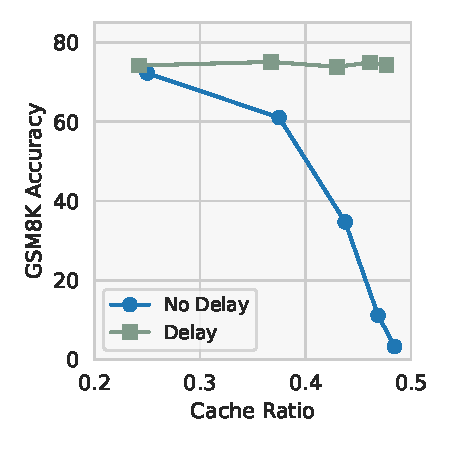
\includegraphics[width=\linewidth]{figure/delay_v3.pdf}
        \captionof{figure}{Effect of one-step delayed caching}
        \label{fig:timestep-delay}
    \end{minipage}
\end{figure}



\subsection{Analysis}

\paragraph{The one-step delay in \methodname.} 
Figure~\ref{fig:timestep-delay} illustrates the impact of applying a one-step delay to the cache mechanism. Without the delay, performance remains acceptable at low cache ratios but degrades rapidly as the cache ratio increases, ultimately collapsing to near-zero accuracy. In contrast, introducing a one-step delay stabilizes the generation quality, enabling the model to maintain nearly lossless performance even under high cache ratios.

\paragraph{Performance on different decoding length, denoising steps and refreshing steps.} Figure~\ref{fig:length_refresh} presents the results of applying \dmethodname\ and \mmethodname\ under various configurations, including different decoding lengths, refresh intervals, sampling steps, and window sizes. Overall, our method consistently achieves performance comparable to the original model without \methodname, effectively pushing the Pareto front forward.
We observe the following findings:
(1) Decoding robustness: The performance impact of our method is largely insensitive to the number of decoding steps, indicating strong robustness across varying generation lengths and sampling steps.
(2) Enhanced long-form generation: In tasks involving longer outputs (e.g., L = 512), our method outperforms the baseline, even improving generation quality from 80.97\% to 83.13\% on GSM8K and from 39.63\% to 46.34\% for HumanEval. The results imply a potential inefficiency in how bidirectional attention aggregates contextual signals, pointing to redundancy or underutilization in long-context modeling.
(3) Effectiveness with only a few refreshing: Even with infrequent refreshes (e.g., every 16 steps), the performance degradation remains small.
(4) Effectiveness of local windows: Incorporating a local window notably enhances the performance of \mmethodname\ with minimal additional computational cost.

\paragraph{Memory and speed analysis.} We analyze the speed and memory footprint of \dmethodname\ and \mmethodname\ across varying decoding and prefill lengths. Our method achieves substantial inference acceleration, ranging from 1.75$\times$ to 3.3$\times$, while introducing only a modest increase in memory usage.
Notably, \mmethodname\ demonstrates greater potential for accelerating inference while \dmethodname\ would be capped. In our main experiments, we observed that setting the refresh interval larger than 2 for \mmethodname\ may degrade performance. However, under the same refresh interval, \mmethodname\ consistently achieves higher speedups than \dmethodname, highlighting its potential advantage when refresh frequency is relaxed.


\begin{figure}
    \centering
    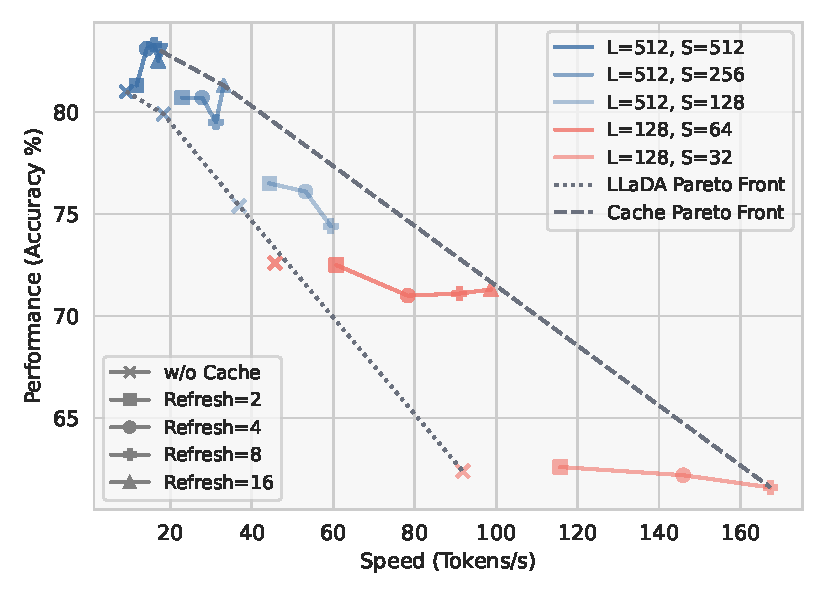
\includegraphics[width=0.47\linewidth]{figure/main_res_v3.pdf}
    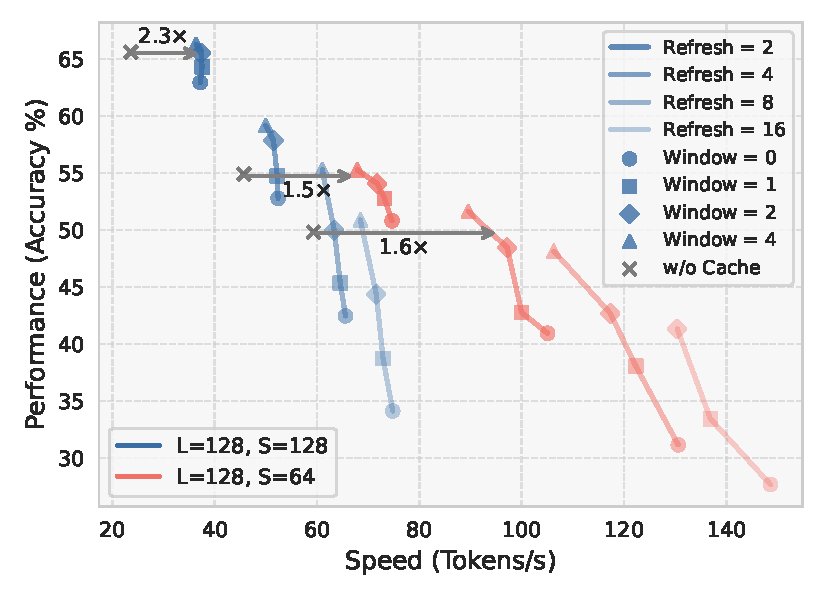
\includegraphics[width=0.47\linewidth]{figure/mask_res_v3.pdf}
    \caption{\dmethodname(left) and \mmethodname(right) on GSM8K with different settings: decoding length $L$, sampling steps $S$, refresh intervals and the window size.}
    \label{fig:length_refresh}
\end{figure}

\begin{figure}
    \centering
    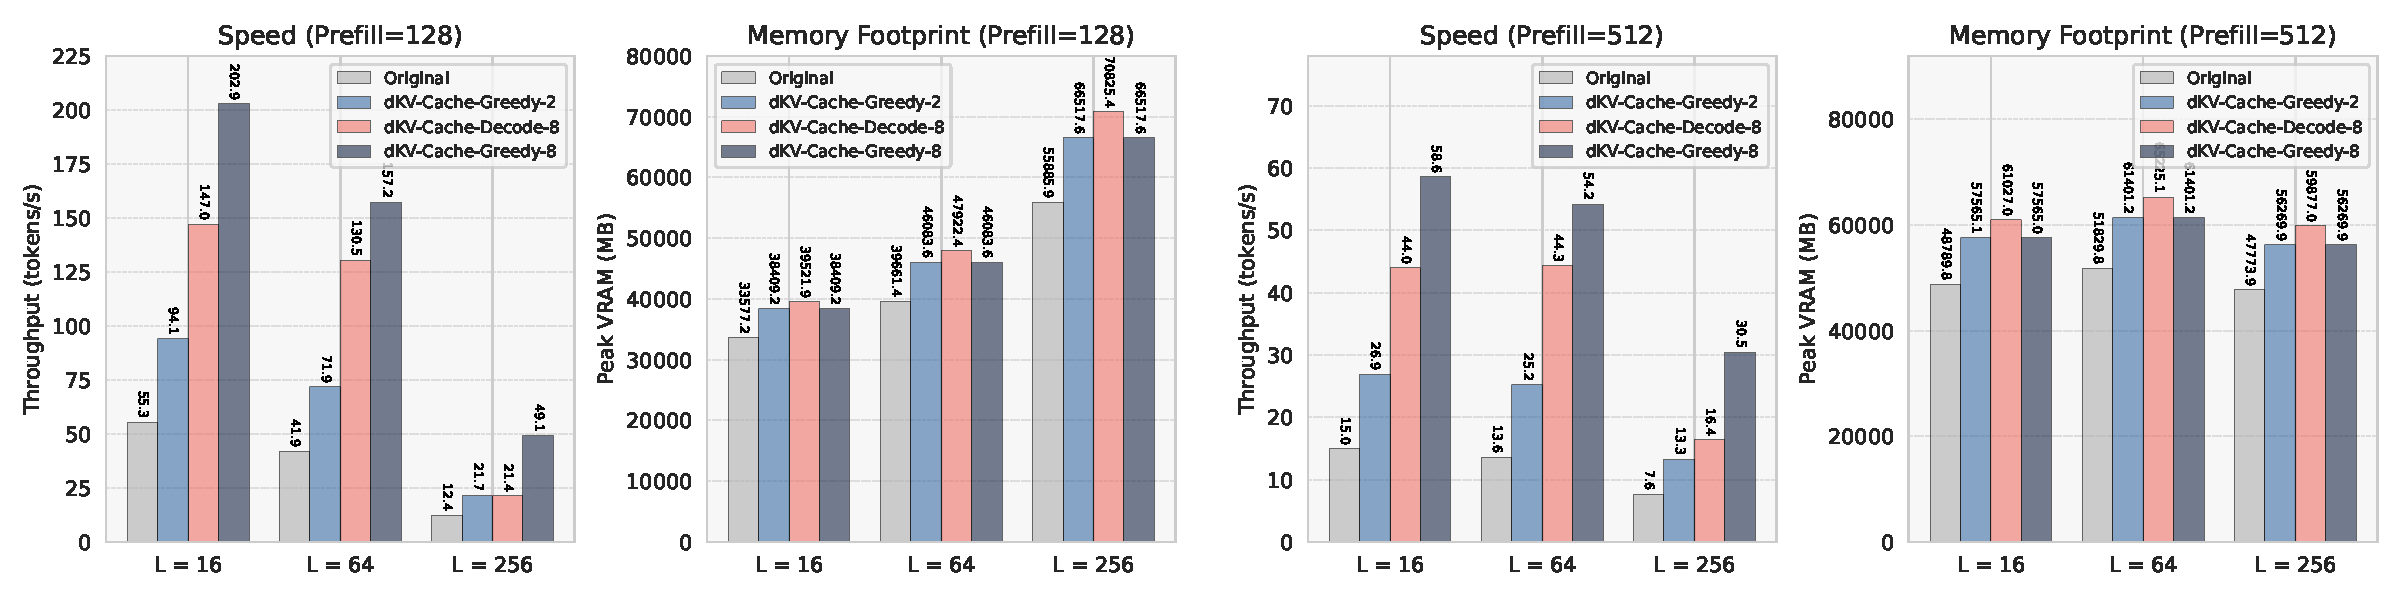
\includegraphics[width=\linewidth]{figure/speed_mem.pdf}
    \caption{Speed and memory for \dmethodname\ and \mmethodname. The number (2 and 8) means that in every n steps, the cache would be refreshed.}
    \label{fig:enter-label}
\end{figure}


\section{Conclusions and Limitations}
In this work, we explore the feasibility of incorporating the caching mechanism into diffusion language models. Specifically, we propose a delayed KV-Cache for DLMs, motivated by our empirical observations on the dynamics of the token representations throughout the diffusion process. Building on this insight, we introduce two cache variants, \dmethodname\ and \mmethodname, each designed to leverage delayed caching for improved compatibility with diffusion-based generation. Our analysis reveals that introducing a delay is crucial for the cache to function effectively in this setting. Extensive experiments demonstrate that our approach largely accelerates inference while maintaining model performance.

One primary limitation of this work lies in its focus on algorithmic design in isolation. While our proposed method introduces an effective caching mechanism from a purely algorithmic perspective, diffusion language models also exhibit substantial room for improvement at the system level. We believe that future research integrating algorithmic innovations with system-level optimization, such as memory management, parallelism, and hardware-aware execution, could unlock further efficiency gains and performance improvements for DLMs.

\medskip

\clearpage
{
\small
\bibliographystyle{plain}
\bibliography{citation}
}

%%%%%%%%%%%%%%%%%%%%%%%%%%%%%%%%%%%%%%%%%%%%%%%%%%%%%%%%%%%%
\iffalse
\newpage
\section*{NeurIPS Paper Checklist}

\begin{enumerate}

\item {\bf Claims}
    \item[] Question: Do the main claims made in the abstract and introduction accurately reflect the paper's contributions and scope?
    \item[] Answer: \answerYes{} % Replace by \answerYes{}, \answerNo{}, or \answerNA{}.
    \item[] Justification: The abstract and introduction clearly state the claims made, and experiments are conducted to support those claims.
    \item[] Guidelines:
    \begin{itemize}
        \item The answer NA means that the abstract and introduction do not include the claims made in the paper.
        \item The abstract and/or introduction should clearly state the claims made, including the contributions made in the paper and important assumptions and limitations. A No or NA answer to this question will not be perceived well by the reviewers. 
        \item The claims made should match theoretical and experimental results, and reflect how much the results can be expected to generalize to other settings. 
        \item It is fine to include aspirational goals as motivation as long as it is clear that these goals are not attained by the paper. 
    \end{itemize}

\item {\bf Limitations}
    \item[] Question: Does the paper discuss the limitations of the work performed by the authors?
    \item[] Answer: \answerYes{} % Replace by \answerYes{}, \answerNo{}, or \answerNA{}.
    \item[] Justification: In Section 5.
    \item[] Guidelines:
    \begin{itemize}
        \item The answer NA means that the paper has no limitation while the answer No means that the paper has limitations, but those are not discussed in the paper. 
        \item The authors are encouraged to create a separate "Limitations" section in their paper.
        \item The paper should point out any strong assumptions and how robust the results are to violations of these assumptions (e.g., independence assumptions, noiseless settings, model well-specification, asymptotic approximations only holding locally). The authors should reflect on how these assumptions might be violated in practice and what the implications would be.
        \item The authors should reflect on the scope of the claims made, e.g., if the approach was only tested on a few datasets or with a few runs. In general, empirical results often depend on implicit assumptions, which should be articulated.
        \item The authors should reflect on the factors that influence the performance of the approach. For example, a facial recognition algorithm may perform poorly when image resolution is low or images are taken in low lighting. Or a speech-to-text system might not be used reliably to provide closed captions for online lectures because it fails to handle technical jargon.
        \item The authors should discuss the computational efficiency of the proposed algorithms and how they scale with dataset size.
        \item If applicable, the authors should discuss possible limitations of their approach to address problems of privacy and fairness.
        \item While the authors might fear that complete honesty about limitations might be used by reviewers as grounds for rejection, a worse outcome might be that reviewers discover limitations that aren't acknowledged in the paper. The authors should use their best judgment and recognize that individual actions in favor of transparency play an important role in developing norms that preserve the integrity of the community. Reviewers will be specifically instructed to not penalize honesty concerning limitations.
    \end{itemize}

\item {\bf Theory assumptions and proofs}
    \item[] Question: For each theoretical result, does the paper provide the full set of assumptions and a complete (and correct) proof?
    \item[] Answer: \answerNA % Replace by \answerYes{}, \answerNo{}, or \answerNA{}.
    \item[] Justification: No theory is proposed in the paper.
    \item[] Guidelines:
    \begin{itemize}
        \item The answer NA means that the paper does not include theoretical results. 
        \item All the theorems, formulas, and proofs in the paper should be numbered and cross-referenced.
        \item All assumptions should be clearly stated or referenced in the statement of any theorems.
        \item The proofs can either appear in the main paper or the supplemental material, but if they appear in the supplemental material, the authors are encouraged to provide a short proof sketch to provide intuition. 
        \item Inversely, any informal proof provided in the core of the paper should be complemented by formal proofs provided in appendix or supplemental material.
        \item Theorems and Lemmas that the proof relies upon should be properly referenced. 
    \end{itemize}

    \item {\bf Experimental result reproducibility}
    \item[] Question: Does the paper fully disclose all the information needed to reproduce the main experimental results of the paper to the extent that it affects the main claims and/or conclusions of the paper (regardless of whether the code and data are provided or not)?
    \item[] Answer: \answerYes{} % Replace by \answerYes{}, \answerNo{}, or \answerNA{}.
    \item[] Justification: Experimental details are listed in Section 4.1 and the Appendix.
    \item[] Guidelines:
    \begin{itemize}
        \item The answer NA means that the paper does not include experiments.
        \item If the paper includes experiments, a No answer to this question will not be perceived well by the reviewers: Making the paper reproducible is important, regardless of whether the code and data are provided or not.
        \item If the contribution is a dataset and/or model, the authors should describe the steps taken to make their results reproducible or verifiable. 
        \item Depending on the contribution, reproducibility can be accomplished in various ways. For example, if the contribution is a novel architecture, describing the architecture fully might suffice, or if the contribution is a specific model and empirical evaluation, it may be necessary to either make it possible for others to replicate the model with the same dataset, or provide access to the model. In general. releasing code and data is often one good way to accomplish this, but reproducibility can also be provided via detailed instructions for how to replicate the results, access to a hosted model (e.g., in the case of a large language model), releasing of a model checkpoint, or other means that are appropriate to the research performed.
        \item While NeurIPS does not require releasing code, the conference does require all submissions to provide some reasonable avenue for reproducibility, which may depend on the nature of the contribution. For example
        \begin{enumerate}
            \item If the contribution is primarily a new algorithm, the paper should make it clear how to reproduce that algorithm.
            \item If the contribution is primarily a new model architecture, the paper should describe the architecture clearly and fully.
            \item If the contribution is a new model (e.g., a large language model), then there should either be a way to access this model for reproducing the results or a way to reproduce the model (e.g., with an open-source dataset or instructions for how to construct the dataset).
            \item We recognize that reproducibility may be tricky in some cases, in which case authors are welcome to describe the particular way they provide for reproducibility. In the case of closed-source models, it may be that access to the model is limited in some way (e.g., to registered users), but it should be possible for other researchers to have some path to reproducing or verifying the results.
        \end{enumerate}
    \end{itemize}


\item {\bf Open access to data and code}
    \item[] Question: Does the paper provide open access to the data and code, with sufficient instructions to faithfully reproduce the main experimental results, as described in supplemental material?
    \item[] Answer: \answerYes{} % Replace by \answerYes{}, \answerNo{}, or \answerNA{}.
    \item[] Justification: The code would be submitted in the supplementary files and we would release the code.
    \item[] Guidelines:
    \begin{itemize}
        \item The answer NA means that paper does not include experiments requiring code.
        \item Please see the NeurIPS code and data submission guidelines (\url{https://nips.cc/public/guides/CodeSubmissionPolicy}) for more details.
        \item While we encourage the release of code and data, we understand that this might not be possible, so “No” is an acceptable answer. Papers cannot be rejected simply for not including code, unless this is central to the contribution (e.g., for a new open-source benchmark).
        \item The instructions should contain the exact command and environment needed to run to reproduce the results. See the NeurIPS code and data submission guidelines (\url{https://nips.cc/public/guides/CodeSubmissionPolicy}) for more details.
        \item The authors should provide instructions on data access and preparation, including how to access the raw data, preprocessed data, intermediate data, and generated data, etc.
        \item The authors should provide scripts to reproduce all experimental results for the new proposed method and baselines. If only a subset of experiments are reproducible, they should state which ones are omitted from the script and why.
        \item At submission time, to preserve anonymity, the authors should release anonymized versions (if applicable).
        \item Providing as much information as possible in supplemental material (appended to the paper) is recommended, but including URLs to data and code is permitted.
    \end{itemize}


\item {\bf Experimental setting/details}
    \item[] Question: Does the paper specify all the training and test details (e.g., data splits, hyperparameters, how they were chosen, type of optimizer, etc.) necessary to understand the results?
    \item[] Answer: \answerYes{} % Replace by \answerYes{}, \answerNo{}, or \answerNA{}.
    \item[] Justification: Experimental details are listed in Section 4.1 and the Appendix.
    \item[] Guidelines:
    \begin{itemize}
        \item The answer NA means that the paper does not include experiments.
        \item The experimental setting should be presented in the core of the paper to a level of detail that is necessary to appreciate the results and make sense of them.
        \item The full details can be provided either with the code, in appendix, or as supplemental material.
    \end{itemize}

\item {\bf Experiment statistical significance}
    \item[] Question: Does the paper report error bars suitably and correctly defined or other appropriate information about the statistical significance of the experiments?
    \item[] Answer: \answerNo{} % Replace by \answerYes{}, \answerNo{}, or \answerNA{}.
    \item[] Justification: No training is involved in the paper.
    \item[] Guidelines:
    \begin{itemize}
        \item The answer NA means that the paper does not include experiments.
        \item The authors should answer "Yes" if the results are accompanied by error bars, confidence intervals, or statistical significance tests, at least for the experiments that support the main claims of the paper.
        \item The factors of variability that the error bars are capturing should be clearly stated (for example, train/test split, initialization, random drawing of some parameter, or overall run with given experimental conditions).
        \item The method for calculating the error bars should be explained (closed form formula, call to a library function, bootstrap, etc.)
        \item The assumptions made should be given (e.g., Normally distributed errors).
        \item It should be clear whether the error bar is the standard deviation or the standard error of the mean.
        \item It is OK to report 1-sigma error bars, but one should state it. The authors should preferably report a 2-sigma error bar than state that they have a 96\% CI, if the hypothesis of Normality of errors is not verified.
        \item For asymmetric distributions, the authors should be careful not to show in tables or figures symmetric error bars that would yield results that are out of range (e.g. negative error rates).
        \item If error bars are reported in tables or plots, The authors should explain in the text how they were calculated and reference the corresponding figures or tables in the text.
    \end{itemize}

\item {\bf Experiments compute resources}
    \item[] Question: For each experiment, does the paper provide sufficient information on the computer resources (type of compute workers, memory, time of execution) needed to reproduce the experiments?
    \item[] Answer: \answerYes{} % Replace by \answerYes{}, \answerNo{}, or \answerNA{}.
    \item[] Justification: In section 4.
    \item[] Guidelines:
    \begin{itemize}
        \item The answer NA means that the paper does not include experiments.
        \item The paper should indicate the type of compute workers CPU or GPU, internal cluster, or cloud provider, including relevant memory and storage.
        \item The paper should provide the amount of compute required for each of the individual experimental runs as well as estimate the total compute. 
        \item The paper should disclose whether the full research project required more compute than the experiments reported in the paper (e.g., preliminary or failed experiments that didn't make it into the paper). 
    \end{itemize}
    
\item {\bf Code of ethics}
    \item[] Question: Does the research conducted in the paper conform, in every respect, with the NeurIPS Code of Ethics \url{https://neurips.cc/public/EthicsGuidelines}?
    \item[] Answer: \answerYes{} % Replace by \answerYes{}, \answerNo{}, or \answerNA{}.
    \item[] Justification: The research conforms to the NeurIPS Code of Ethics.
    \item[] Guidelines:
    \begin{itemize}
        \item The answer NA means that the authors have not reviewed the NeurIPS Code of Ethics.
        \item If the authors answer No, they should explain the special circumstances that require a deviation from the Code of Ethics.
        \item The authors should make sure to preserve anonymity (e.g., if there is a special consideration due to laws or regulations in their jurisdiction).
    \end{itemize}


\item {\bf Broader impacts}
    \item[] Question: Does the paper discuss both potential positive societal impacts and negative societal impacts of the work performed?
    \item[] Answer: \answerYes{} % Replace by \answerYes{}, \answerNo{}, or \answerNA{}.
    \item[] Justification: In Appendix
    \item[] Guidelines:
    \begin{itemize}
        \item The answer NA means that there is no societal impact of the work performed.
        \item If the authors answer NA or No, they should explain why their work has no societal impact or why the paper does not address societal impact.
        \item Examples of negative societal impacts include potential malicious or unintended uses (e.g., disinformation, generating fake profiles, surveillance), fairness considerations (e.g., deployment of technologies that could make decisions that unfairly impact specific groups), privacy considerations, and security considerations.
        \item The conference expects that many papers will be foundational research and not tied to particular applications, let alone deployments. However, if there is a direct path to any negative applications, the authors should point it out. For example, it is legitimate to point out that an improvement in the quality of generative models could be used to generate deepfakes for disinformation. On the other hand, it is not needed to point out that a generic algorithm for optimizing neural networks could enable people to train models that generate Deepfakes faster.
        \item The authors should consider possible harms that could arise when the technology is being used as intended and functioning correctly, harms that could arise when the technology is being used as intended but gives incorrect results, and harms following from (intentional or unintentional) misuse of the technology.
        \item If there are negative societal impacts, the authors could also discuss possible mitigation strategies (e.g., gated release of models, providing defenses in addition to attacks, mechanisms for monitoring misuse, mechanisms to monitor how a system learns from feedback over time, improving the efficiency and accessibility of ML).
    \end{itemize}
    
\item {\bf Safeguards}
    \item[] Question: Does the paper describe safeguards that have been put in place for responsible release of data or models that have a high risk for misuse (e.g., pretrained language models, image generators, or scraped datasets)?
    \item[] Answer: \answerNA{} % Replace by \answerYes{}, \answerNo{}, or \answerNA{}.
    \item[] Justification: The research poses no such risks.
    \item[] Guidelines:
    \begin{itemize}
        \item The answer NA means that the paper poses no such risks.
        \item Released models that have a high risk for misuse or dual-use should be released with necessary safeguards to allow for controlled use of the model, for example by requiring that users adhere to usage guidelines or restrictions to access the model or implementing safety filters. 
        \item Datasets that have been scraped from the Internet could pose safety risks. The authors should describe how they avoided releasing unsafe images.
        \item We recognize that providing effective safeguards is challenging, and many papers do not require this, but we encourage authors to take this into account and make a best faith effort.
    \end{itemize}

\item {\bf Licenses for existing assets}
    \item[] Question: Are the creators or original owners of assets (e.g., code, data, models), used in the paper, properly credited and are the license and terms of use explicitly mentioned and properly respected?
    \item[] Answer: \answerYes{} % Replace by \answerYes{}, \answerNo{}, or \answerNA{}.
    \item[] Justification: They are properly cited and the license and terms of use are properly respected.
    \item[] Guidelines:
    \begin{itemize}
        \item The answer NA means that the paper does not use existing assets.
        \item The authors should cite the original paper that produced the code package or dataset.
        \item The authors should state which version of the asset is used and, if possible, include a URL.
        \item The name of the license (e.g., CC-BY 4.0) should be included for each asset.
        \item For scraped data from a particular source (e.g., website), the copyright and terms of service of that source should be provided.
        \item If assets are released, the license, copyright information, and terms of use in the package should be provided. For popular datasets, \url{paperswithcode.com/datasets} has curated licenses for some datasets. Their licensing guide can help determine the license of a dataset.
        \item For existing datasets that are re-packaged, both the original license and the license of the derived asset (if it has changed) should be provided.
        \item If this information is not available online, the authors are encouraged to reach out to the asset's creators.
    \end{itemize}

\item {\bf New assets}
    \item[] Question: Are new assets introduced in the paper well documented and is the documentation provided alongside the assets?
    \item[] Answer: \answerNA{} % Replace by \answerYes{}, \answerNo{}, or \answerNA{}.
    \item[] Justification: The paper does not release new assets.
    \item[] Guidelines:
    \begin{itemize}
        \item The answer NA means that the paper does not release new assets.
        \item Researchers should communicate the details of the dataset/code/model as part of their submissions via structured templates. This includes details about training, license, limitations, etc. 
        \item The paper should discuss whether and how consent was obtained from people whose asset is used.
        \item At submission time, remember to anonymize your assets (if applicable). You can either create an anonymized URL or include an anonymized zip file.
    \end{itemize}

\item {\bf Crowdsourcing and research with human subjects}
    \item[] Question: For crowdsourcing experiments and research with human subjects, does the paper include the full text of instructions given to participants and screenshots, if applicable, as well as details about compensation (if any)? 
    \item[] Answer: \answerNA{} % Replace by \answerYes{}, \answerNo{}, or \answerNA{}.
    \item[] Justification: The paper does not involve crowdsourcing nor research with human subjects.
    \item[] Guidelines:
    \begin{itemize}
        \item The answer NA means that the paper does not involve crowdsourcing nor research with human subjects.
        \item Including this information in the supplemental material is fine, but if the main contribution of the paper involves human subjects, then as much detail as possible should be included in the main paper. 
        \item According to the NeurIPS Code of Ethics, workers involved in data collection, curation, or other labor should be paid at least the minimum wage in the country of the data collector. 
    \end{itemize}

\item {\bf Institutional review board (IRB) approvals or equivalent for research with human subjects}
    \item[] Question: Does the paper describe potential risks incurred by study participants, whether such risks were disclosed to the subjects, and whether Institutional Review Board (IRB) approvals (or an equivalent approval/review based on the requirements of your country or institution) were obtained?
    \item[] Answer: \answerNA{} % Replace by \answerYes{}, \answerNo{}, or \answerNA{}.
    \item[] Justification: The paper does not involve crowdsourcing nor research with human subjects.
    \item[] Guidelines:
    \begin{itemize}
        \item The answer NA means that the paper does not involve crowdsourcing nor research with human subjects.
        \item Depending on the country in which research is conducted, IRB approval (or equivalent) may be required for any human subjects research. If you obtained IRB approval, you should clearly state this in the paper. 
        \item We recognize that the procedures for this may vary significantly between institutions and locations, and we expect authors to adhere to the NeurIPS Code of Ethics and the guidelines for their institution. 
        \item For initial submissions, do not include any information that would break anonymity (if applicable), such as the institution conducting the review.
    \end{itemize}

\item {\bf Declaration of LLM usage}
    \item[] Question: Does the paper describe the usage of LLMs if it is an important, original, or non-standard component of the core methods in this research? Note that if the LLM is used only for writing, editing, or formatting purposes and does not impact the core methodology, scientific rigorousness, or originality of the research, declaration is not required.
    %this research? 
    \item[] Answer: \answerNA{} % Replace by \answerYes{}, \answerNo{}, or \answerNA{}.
    \item[] Justification: The core method development in this research does not involve LLMs as any important, original, or non-standard components.
    \item[] Guidelines:
    \begin{itemize}
        \item The answer NA means that the core method development in this research does not involve LLMs as any important, original, or non-standard components.
        \item Please refer to our LLM policy (\url{https://neurips.cc/Conferences/2025/LLM}) for what should or should not be described.
    \end{itemize}

\end{enumerate}
\fi 
\clearpage
\appendix


\section{Design for $\operatorname{concat\_{reorder}}$}

$\operatorname{concat\_{reorder}}$ is our implementation of \methodname\ designed to improve the speed of dKV-Cache in diffusion language models.
Unlike standard KV-Cache used in autoregressive models, \methodname\ requires gathering and scattering keys and values from arbitrary positions, introducing indexing operations that are less efficient than the simple concatenation in contiguous space used in ARs.

In dKV-Cache, the cache process involves two additional indexing operations:
(1) At the cache step: After computing keys and values, we need to gather the corresponding states of cached tokens at non-continuous positions.
(2) At the reuse step: to obtain the whole matrices for key and value, we need to scatter these vectors back to their original positions in the sequence.
In contrast, KV-Cache in ARs only requires matrix slicing and concatenation, making it significantly more efficient.

To minimize the overhead of gathering and scattering, we propose an algorithm similar to that of standard KV-Cache to avoid too many indexing operations. 
The key idea is to reorder token positions during the forward calculation of the Transformer, placing all cached tokens contiguously on one side (e.g., left) and newly decoded tokens on the other. 
This allows us to move parts of the indexing operation to the token level (matrices with shape [B, L]) instead of the intermediate states (matrices with shape [B, L, D]):
\begin{itemize}
    \item At Step t-1: Gather the cached key $\mathbf{K}_{t-1}^{\mathcal{I}\setminus\mathcal{M}_{t-1}}$ and value states $\mathbf{V}_{t-1}^{\mathcal{I}\setminus\mathcal{M}_{t-1}}$ based on the position index $\mathcal{I}\setminus\mathcal{M}_{t-1}$ with one indexing operation.
    \item At Step t: Reorder the sequence, making the cached tokens (at position $\mathcal{I}\setminus\mathcal{M}_{t-1}$) at the left, and uncached tokens (at position $\mathcal{M}_{t-1}$) at the right.
    \item At Step t: Using $\operatorname{concat\_{reorder}}$ for $\left(\mathbf{K}_{t-1}^{\mathcal{I}\setminus\mathcal{M}_{t-1}}, \mathbf{K}_{t}^{\mathcal{M}_{t-1}}\right)$ and for $\left(\mathbf{V}_{t-1}^{\mathcal{I}\setminus\mathcal{M}_{t-1}}, \mathbf{V}_{t}^{\mathcal{M}_{t-1}}\right)$: 
    First, concatenate the cached and current key/value states directly without further gathering/scattering (\textbf{concat}, for getting all K and V to calculate attention), 
    and reorder the whole KV matrics based on $\mathbf{V}_{t}^{\mathcal{I}\setminus\mathcal{M}_{t}}$ to get the cached states for the next step (\textbf{reorder}, for obtaining the cache).
\end{itemize}
The reorder operation is to know the position mapping from $[\mathcal{I}\setminus\mathcal{M}_{t-1}; \mathcal{M}_{t-1}]$ to $[\mathcal{I}\setminus\mathcal{M}_{t}; \mathcal{M}_{t}]$. 
For example, if the unmasked position at $t-1$ is [2, 4, 5] from a sequence of 8 tokens, and at step $t+1$ is [2, 4, 5, 7].
Then $[\mathcal{I}\setminus\mathcal{M}_{t-1}; \mathcal{M}_{t-1}]$ would be [2, 4, 5, 0, 1, 3, 6, 7], and $[\mathcal{I}\setminus\mathcal{M}_{t}; \mathcal{M}_{t}]$ would be [2, 4, 5, 7, 0, 1, 3, 6].
The mapping would be [0, 1, 2, 7, 3, 4, 5, 6], and we only need to get the corresponding entries [0, 1, 2, 7] from $\left[\mathbf{K}_{t-1}^{\mathcal{I}\setminus\mathcal{M}_{t-1}}; \mathbf{K}_{t}^{\mathcal{M}_{t-1}}\right]$ and $\left[\mathbf{V}_{t-1}^{\mathcal{I}\setminus\mathcal{M}_{t-1}}; \mathbf{V}_{t}^{\mathcal{M}_{t-1}}\right]$.

The only remaining thing is that the change of token position would impact the positional encoding. 
However, this is easy to solve; we can also reorder the positional embedding.
Reordering positional embeddings is required only once per model evaluation and can be shared across layers, thus, it would not cost much time.

Furthermore, since our method introduces a one-step shift in caching, the position of cached tokens at step $t$ corresponds to the token positions decoded from step $t-1$. This alignment allows us to track which key and value entries need to be cached without storing the entire key/value matrices, which, to cache which tokens, can only be known after the decoding results at step $t$. 

We present the pseudo-algorithm of our approach in Algorithm ~\ref{ag:concat_reorder}. While it largely improves inference speed over the naive implementation, the concat and reorder operations still introduce some overhead. We believe there is substantial potential for further optimization.

\begin{algorithm}[htbp!]
\caption{Pseudo code for \dmethodname. We take step t as an example.} \label{ag:concat_reorder}
\begin{algorithmic}[1]
\Require Sequence $\bx_{c(t)}^{1:L}$ at step $t$ (Simplied as $\bx$), position index of masked tokens $\mathcal{M}_{t}$, cached Key  $\mathbf{K}_{t-1}^{\mathcal{I}\setminus\mathcal{M}_{t-1}}$ and Value $\mathbf{V}_{t-1}^{\mathcal{I}\setminus\mathcal{M}_{t-1}}$
%
%\State $(K_{\mathrm{all}},\,V_{\mathrm{all}}) \gets \mathrm{ComputeKV}(x_t^{1:L})$
%\Comment{compute all K/V at step $t$}
%\State $K_{\mathrm{cache}}\gets K_{\mathrm{all}}[\,1:D_{\mathrm{prev}}\,]$
%\State $V_{\mathrm{cache}}\gets V_{\mathrm{all}}[\,1:D_{\mathrm{prev}}\,]$
%\medskip
%\Comment{--- Move to step $t+1$ ---}
%\State Let $I_{\mathrm{uncached}}\gets \{D_{\mathrm{prev}}+1,\dots,L\}$

\State $\bx^\prime \gets  \bx[\mathcal{M}_{t-1}]$ \Comment{$\mathcal{M}_{t-1}$: $t-1$ for one-step shift}
\State $\textbf{PE}^\prime\;\gets\;\bigl[\textbf{PE}_{}[\mathcal{I}\setminus\mathcal{M}_{t-1}]\;;\;\textbf{PE}_{}[\mathcal{M}_{t-1}]\bigr]$
\Comment{\small Positional embeddings: cached on left, uncached on right}
\State $\mathbf{Q}_t^{\mathcal{M}_t}, \mathbf{K}_t^{\mathcal{M}_t}, \mathbf{V}_t^{\mathcal{M}_t} \gets \mathcal{T}(\bx^\prime)$ \Comment{$\mathcal{T}$: Calculation in Transformer to get Q, K and V}
\State $\mathbf{K}_t^{\mathcal{I}} \gets \operatorname{Concat}\left(\mathbf{K}_{t-1}^{\mathcal{I}\setminus\mathcal{M}_{t-1}}, \mathbf{K}_t^{\mathcal{M}_{t-1}}\right)$, $\mathbf{V}_t^{\mathcal{I}} \gets \operatorname{Concat}\left(\mathbf{V}_{t-1}^{\mathcal{I}\setminus\mathcal{M}_{t-1}}, \mathbf{V}_t^{\mathcal{M}_{t-1}}\right)$ \Comment{Get all K and V}
\State $\mathbf{K}_t^{\mathcal{I}\setminus\mathcal{M}_{t}} \gets \operatorname{Reorder}(\mathbf{K}_t^{\mathcal{I}}, I^{\prime})$, $\mathbf{V}_t^{\mathcal{I}\setminus\mathcal{M}_{t}} \gets \operatorname{Reorder}(\mathbf{V}_t^{\mathcal{I}}, I^{\prime})$ \Comment{$\mathcal{I^\prime}:$ The index of $\mathcal{I}\setminus\mathcal{M}_t$ in the $\bigl[\bx[\mathcal{I}\setminus\mathcal{M}_{t-1}]\;;\;\bx[\mathcal{M}_{t-1}]\bigr]$}
\State $p^{\prime} \gets \mathcal{A}(\mathbf{Q}_t^{\mathcal{M}_t}, \mathbf{K}_t^{\mathcal{I}}, \mathbf{V}_t^{\mathcal{I}})$  
\State $p \gets \operatorname{Scatter}(p^\prime, \mathcal{M}_{t-1})$ \Comment{Put the token logits back to the original position}
\medskip
\State \textbf{Return} $p$, $\mathbf{K}_t^{\mathcal{I}\setminus\mathcal{M}_{t}}$, $\mathbf{V}_t^{\mathcal{I}\setminus\mathcal{M}_{t}}$
\end{algorithmic}
\end{algorithm}

\section{Design for Dream}

\begin{figure}[htbp!]
    \centering
    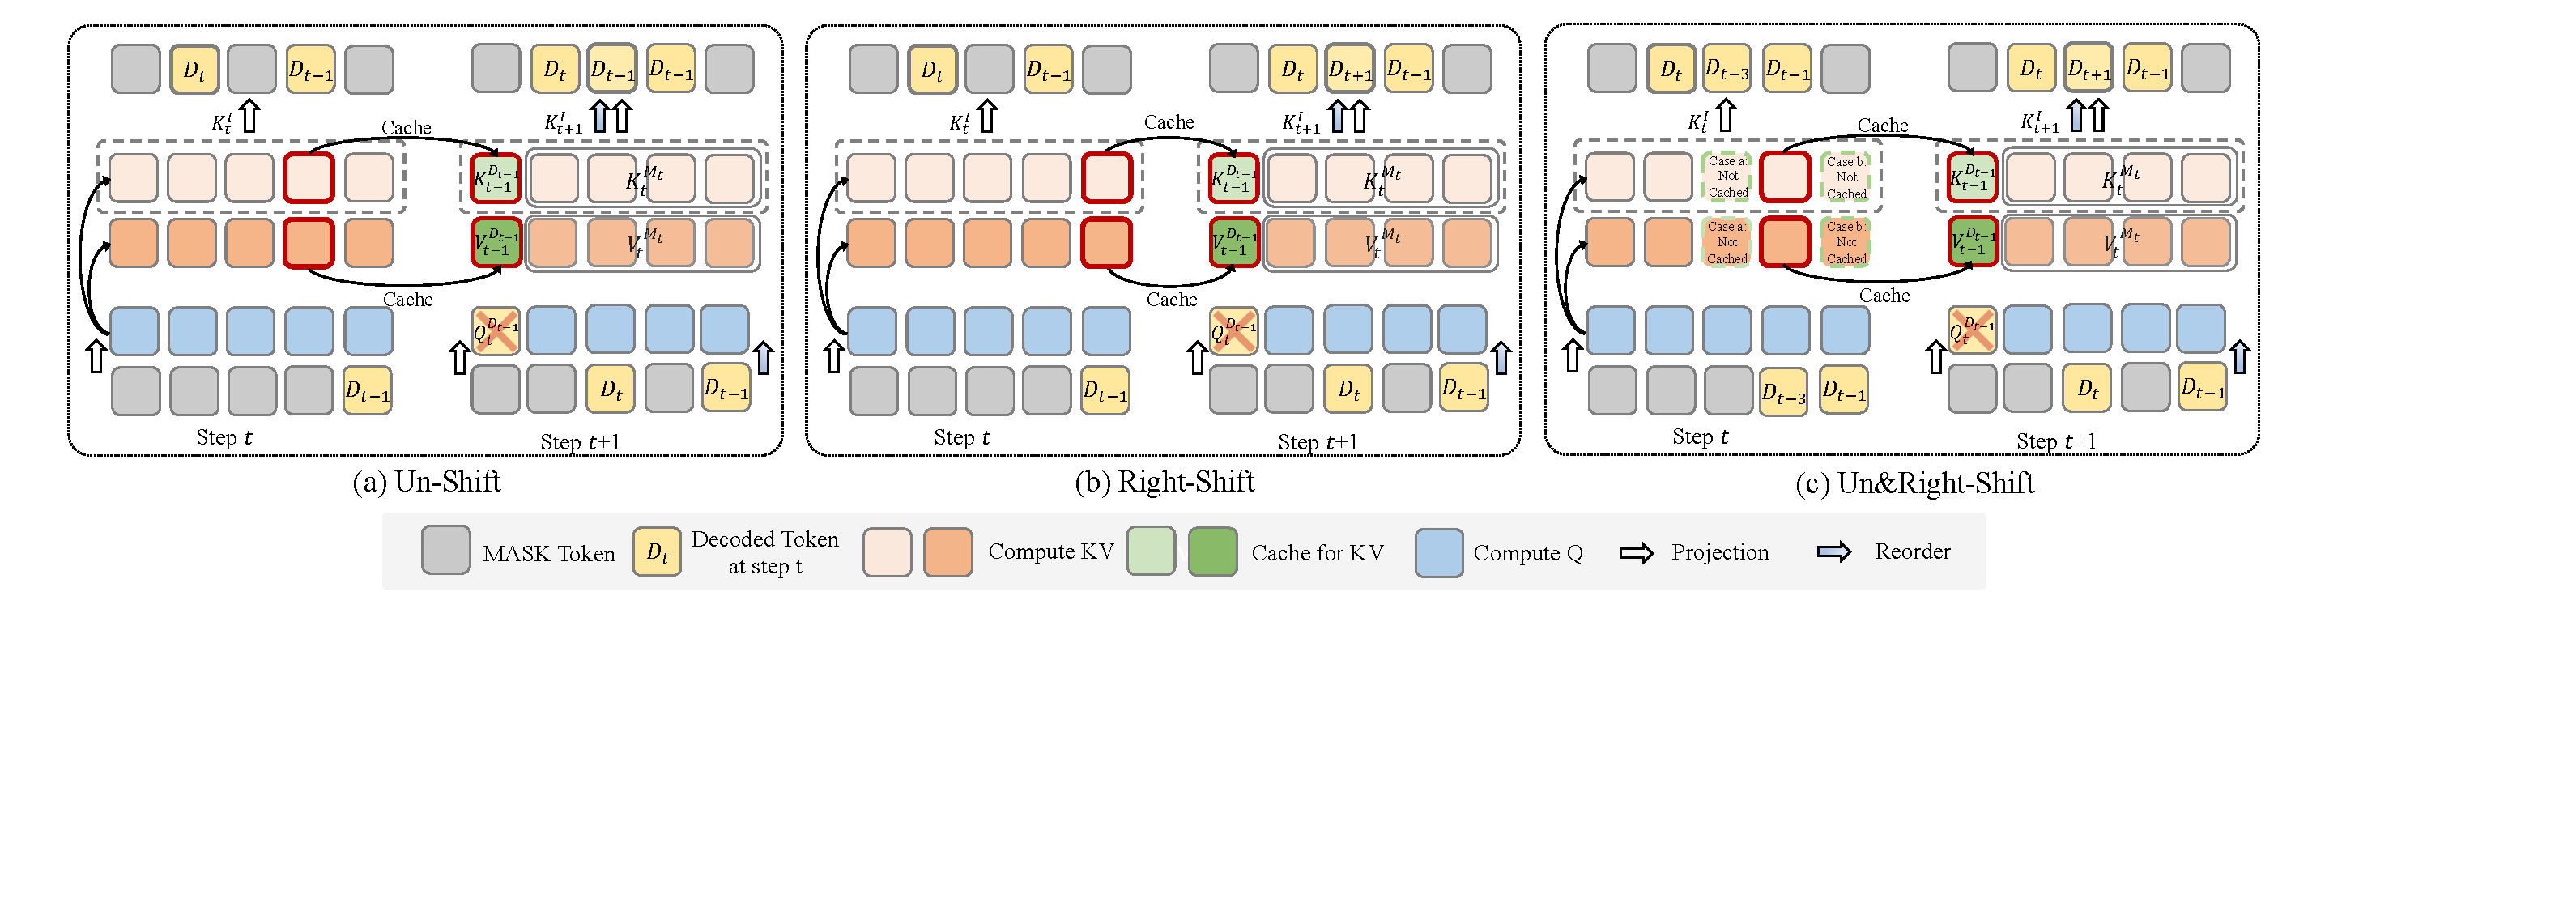
\includegraphics[width=\linewidth]{figure/dream_cache_v3.pdf}
    \caption{Three variants for the caching strategy for diffusion language models adapted from auto-regressive language models, which would have shifted output position.}
    \label{fig:dream_cache_pos}
\end{figure}

Dream has a different caching strategy with LLaDA. The main reason for this is that Dream is adapted from pre-trained autoregressive models, which would make the position of output align with the probability of the next token, instead of the current token in the traditional setting of masked diffusion models. This would make a difference in the caching strategy and we investigate between different designs of those caching strategies:

\begin{itemize}
    \item Un-Shift, Figure \ref{fig:dream_cache_pos}(a): We cache the unshifted token representations. Specifically, for the t-th token, we store its key and value as $\mathbf{K}^{t}$ and $\mathbf{V}^{t}$ at position $t$.
    \item Right-Shift, Figure \ref{fig:dream_cache_pos}(b): Given that the hidden state is highly sensitive to changes in input, we also explore a right-shifted variant. Here, for the t-th token, we cache $\mathbf{K}^{t+1}$ and $\mathbf{V}^{t+1}$. 
    \item Un\&Right-Sift, Figure \ref{fig:dream_cache_pos}(c): We introduce a stricter variant where caching is conditioned on both input stability and decoding completion. For the t-th token, we cache its features only after its input is fixed and it has been decoded.
\end{itemize}

The one-step shift is still used here. For example, in the right-shift variant, the t-th token is fed into the model at position t+1 in the next step, and we cache its output $\mathbf{K}^{t+1}$ and $\mathbf{V}^{t+1}$ then.
The results are shown in Table \ref{tab:dream_shift}, where Un\&right-shift would have the best performance, and the right shift would largely harm the model performance. 
However, we use the Un-Shift in our main experiment, since Un\&right-shift is incompatible with the above $\operatorname{concat\_reorder}$.

\begin{table}[htbp!]
    \centering
    \caption{Comparison between different types of caching strategy for Dream-Base-7B. }
    \label{tab:dream_shift}
    \begin{tabular}{c|ccc}
        \toprule
                      &  Un-Shift  &   Right-Shift &  Un\&Right Shift \\
        \midrule
         MMLU         &  71.78 & 64.60 & 71.73 \\
         GSM8K        &  76.34  & 32.68 & 77.71  \\
        \bottomrule
    \end{tabular}
\end{table}

\section{Evaluation Details}

\subsection{For LLaDA}
We re-implemented the evaluation of LLaDA on those reported datasets. 
We generate and extract the final answer instead of comparing the log prob in the multiple-choice question. 
Thus, the result of MMLU and GPQA is lower than reported since the model sometimes cannot generate the answer in the given format or does not generate the answer. 
We show the configuration of each experiment in Table \ref{tab:config_llada}

\begin{table}[htbp]
    \centering
    \caption{Configurations of experiments on LLaDA-Instruct.} \label{tab:config_llada}
    \resizebox{1.0\linewidth}{!}{
    \begin{tabular}{c||cc|cc||cc}
        \toprule
        & Base & Few-Steps &  \mmethodname & \mmethodname & Half-Steps & \dmethodname \\
        Remasking & \small (random / confidence) & \small (random) & \small (random) & \small (random) & \small (confidence) & \small (confidence) \\
        & Configuration & Steps $T$ & Cache Interval & Window Size & Steps $T$ & Cache Interval \\
        \midrule
        MMLU    &  L=32, T=32, B=16 & T=20 & 2 & 4 & T=16 & 8  \\ % 32, 32, 16         
        \midrule
        GSM8K   & L=256, T=256, B=32 &  T=160 & 2 &  4  & T=128 & 8 \\ 
        Math500  & L=256, T=256, B=64 & T=160 & 2 &  4 & T=128 & 8 \\  
        GPQA      & L=128, T=128, B=64 & T=80 & 2 &  4 & T=64 & 8 \\ 
        \midrule
        HumanEval   & L=512, T=512, B=32 & T=320 & 2 & 4 & T=256 & 8 \\
        MBPP & L=512, T=512, B=32 & T=320 & 2 &  2 & T=256 & 8\\
        \bottomrule
    \end{tabular}
    }
\end{table}

\subsection{For Dream}
We follow the original evaluation pipeline for Dream\footnote{https://github.com/HKUNLP/Dream/blob/main/eval/eval\_dream\_gen.sh} and we also adopt two datasets, MMLU and GPQA, to generate the answer instead of comparing the probabilities. 
We follow all the hyperparameters set in the evaluation script, including the temperature, the remasking strategy, top\_p and the number of few-shot in in-context learning. 

\section{Impact of batch size on speed}
\begin{figure}[htbp]
    \centering
    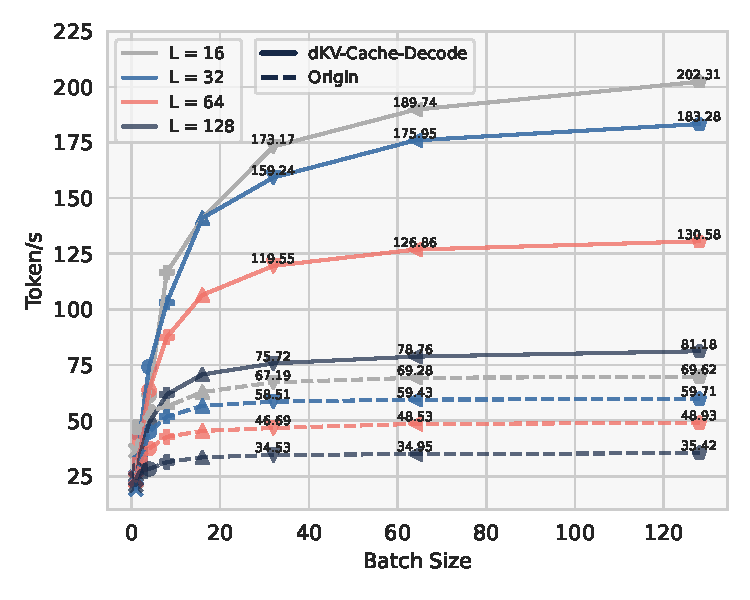
\includegraphics[width=0.5\linewidth]{figure/batch_size_speed_v2.pdf}
    \caption{Impact of batch size on decoding speed. Evaluated on LLaDA with a single NVIDIA H20; prefill length fixed at 100 tokens.}
    \label{fig:batch_size_speed}
\end{figure}

Our inference pipeline relies heavily on indexing operations, gathers and scatters, that generate a stream of small, non-contiguous memory accesses. At a batch size of one, these uncoalesced reads make the inference memory-bound. As a result, the GPU’s compute units sit idle waiting for data. In some cases with the batch size equal to 1, inference with caching can actually underperform the unaccelerated baseline. By contrast, scaling up the batch size can solve this problem and deliver far greater, more stable speed-up ratios over the baseline.

\iffalse
\section{Detailed results of using different caching configurations.}
\begin{table}[htbp!]
    \centering
    \caption{LLaDA results with different L, S and refreshing steps. We use GSM8K to evaluate the performance here. Here, `-` represents we didn't test on this setting since it involves cross-block caching.}
    \resizebox{.6\linewidth}{!}{
    \begin{tabular}{cc|c|ccccc}
    \toprule
        L & S & Base & 2 & 4 & 8 & 16 & 32 \\ 
    \midrule
         \multirow{3}{*}{128} & 128 & 73.77 & 74.15	& 75.06	& 73.84	& 74.90	& 74.30 \\
         & 64  & 72.55	& 72.48	& 70.96	& 71.11	& 71.34	& - \\
         & 32 & 62.40	& 62.62	& 62.24	& 61.64 & - & - \\
    \midrule
         \multirow{3}{*}{256} & 256 & 77.56	& 77.48	& 78.85	& 76.72	& 76.27	& 75.66 \\
         & 128 & 77.91	& 78.01	& 76.11	& 75.96	& 75.36 & - \\
         & 64  & 71.57	& 71.49	& 71.27	& 72.86 & - & -\\
    \midrule
        \multirow{3}{*}{512} & 512 & 80.97	& 81.27	& 83.13	& 83.32 & 82.49	& 83.01  \\
        & 256 & 79.98	& 80.74	& 80.74	& 79.52	& 81.27 & -\\
        & 128 & 75.44	& 76.49	& 76.11	& 74.37 & - & -\\
    \midrule
        1024 & 1024 & 82.11 & 82.49 & 83.61 & 82.03 & 82.94 & 81.96 \\
    \bottomrule
    \end{tabular}
    }
\end{table}
\fi

\section{Case Study}
We provide the case study of our method in Table \ref{tbl:case_study_llada} and Table \ref{tbl:case_study_dream_free} and Table \ref{tbl:case_study_Dream}.

\begin{table}[t]
    \centering
    \caption{Case study on LLaDA-8B-Instruct. Question: Lily can run 12 kilometers per hour for 4 hours. After that, she runs 6 kilometers per hour. How many kilometers can she run in 8 hours?} \label{tbl:case_study_llada}
    \begin{tabular}{p{2cm}|p{10cm}}
    \toprule
    Model & Generate Text (L=128, T=128, B=64)\\
    \midrule
        LLaDA-8B-Instruct (low confidence) & 1. Calculate the distance Lily runs in the first 4 hours:
        
   - Speed: 12 kilometers per hour
   
   - Time: 4 hours
   
   - Distance: 12 km/h * 4 h = 48 km

2. Calculate the distance Lily runs in the next 4 hours:

   - Speed: 6 kilometers per hour
   
   - Time: 4 hours
   
   - Distance: 6 km/h * 4 h = 24 km

3. Add the distances together:

   - Total distance: \textbackslash boxed\{72\} km \\ 

    \midrule
    \dmethodname, Refresh = 4 & 1. Calculate the distance Lily runs in the first 4 hours:
    
   - Distance = Speed × Time = 12 km/h × 4 h = 48 km

2. Calculate the distance Lily runs in the next 4 hours:

   - Distance = Speed × Time = 6 km/h × 4 h = 24 km

3. Add the distances from both periods to find the total distance Lily runs in 8 hours:

   - Total Distance = 48 km + 24 km = 72 km

\textbackslash boxed\{72 km\} \\
    \midrule
   \dmethodname, Refresh=16 & 1. Calculate the distance Lily runs in the first 4 hours: 
   
   12 km/hour * 4 hours = 48 km

2. Calculate the distance Lily runs in the next 4 hours: 

   6 km/hour * 4 hours = 24 km

3. Add the distances from the first 4 hours and the next 4 hours to find the total distance she runs: 

   48 km + 24 km = 72 km

Therefore, Lily can run \textbackslash boxed\{72\} kilometers in 8 hours. \\ 
\midrule

\mmethodname, Refresh = 2 & To determine how many kilometers Lily can run in 8 hours, we need to break down her running schedule and sum the distances.

First, calculate the distance she runs at 12 kilometers per hour for 4 hours:
\[ 12 * 4 = 48\]

After 4 hours, she runs 6 kilometers per hour for the remaining 4 hours:
\[ 6 * 4 = 24\]

Now, add the distances:
\[ 48 + 24 = 72\]

\textbackslash boxed\{72\}  \\
\midrule
\mmethodname, Refresh = 4 (random) & For the first 4 hours Lily runs at 12 kilometers per hour, so she runs 12 * 4 = 48 kilometers.
 8 hours - 4 hours are left after the first 4 (8 - 4 = 4 hours).

For the next 4 hours, she runs at 6 kilometers per hour, so she runs 6 * 4 = 24 kilometers.

Adding the two distances together, Lily can run 48 + 24 = 72 kilometers in 8 hours.

Answer: \textbackslash boxed\{72\}  \\
   \bottomrule
    \end{tabular}
\end{table}


\begin{table}[t]
    \centering
    \caption{Case study on Dream-Instruct-7B. Request: Write a story that ends with "Finally, Joey and Rachel get married."} \label{tbl:case_study_dream_free}
    \begin{tabular}{p{2cm}|p{11cm}}
    \toprule
    Model & Generate Text (L=256, T=256)\\
    \midrule
    Dream-Instruct-7B (Entropy) & Once upon a time, there was a young man named Joey who lived in a small town in the middle of nowhere. He was a kind and gentle soul who loved to sing and play the guitar. One day, he met a beautiful girl named Rachel who was also a talented singer and musician. They fell in love and decided to get married. However, there was a problem. Joey's parents were against the marriage because they didn't know Rachel well enough. They thought that she was not a good match for their son. Rachel, on the other hand, was not worried about Joey's parents' opinion. She knew that she loved Joey and that he was the one for her. She decided to try and win over Joey's parents by showing them how much she cared about him. She started by cooking for them and inviting them to her house for dinner. She also took them on a trip to the mountains where they could enjoy the scenery and the fresh air. After a while, Joey's parents started to see Rachel in a different light. They realized that she was a good person and that she loved Joey very much. They decided to give their blessing to the marriage. Finally, Joey and Rachel got married and lived happily ever after. \\
    \midrule
    \dmethodname, Refresh = 16 & Once upon a time, in a small town called New York, there lived a young man named Joey and a young woman named Rachel. They were both very happy with their lives, but they were also very different from each other. Joey was a very outgoing person who loved to be around people, while Rachel was a very introverted person who loved to be alone. 
One day, Joey and Rachel met at a coffee shop and fell in love. They spent hours talking and laughing together, and they realized that they were perfect for each other. They decided to be together and build their lives together. 
As the years went by, Joey and Rachel grew closer and closer. They shared their dreams and their fears, and they supported each other through thick and thin. They were a perfect match, and they knew that they were meant to be together. 
Finally, Joey and Rachel got married. They had a beautiful wedding with all their friends and family in attendance. They were so happy to be together, and they knew that they would always be together. \\
    \midrule
    \pmethodname & Once upon a time, in a small town called New York, there lived a young man named Joey. Joey was a kind and caring person who always tried to help others. He had a beautiful girlfriend named Rachel, who was also kind and caring. They were in love with each other and wanted to spend their lives together.
One day, Joey and Rachel decided to get married. They planned their wedding for a long time, and everyone in the town was excited to attend. On the day of the wedding, Joey and Rachel exchanged vows and promised to love each other forever.
After the wedding, Joey and Rachel moved into a beautiful house in the countryside. They were happy and content with their lives, and they had two children, a boy and a girl. The children grew up to be kind and caring people, just like their parents.
As the years went by, Joey and Rachel continued to love each other deeply. They had many ups and downs, but they always found a way to overcome their challenges and stay together.
Finally, after many years of marriage, Joey and Rachel decided to retire and live in a small cottage in the countryside. They were happy and content with their lives, and they knew that they had found the love of their lives in each other.\\
    \bottomrule
    \end{tabular}
\end{table}


\begin{table}[t!]
    \centering
    \caption{Case study on Dream-Instruct-7B. Question: Lily can run 12 kilometers per hour for 4 hours. After that, she runs 6 kilometers per hour. How many kilometers can she run in 8 hours?} \label{tbl:case_study_Dream}
    \begin{tabular}{p{2cm}|p{11cm}}
    \toprule
    Model & Generate Text (L=128, T=128)\\
    \bottomrule
    Dream-Instruct-7B (Entropy) & In the first 4 hours, Lily runs 12 kilometers per hour, so she runs a total of 12 * 4 = 48 kilometers.
In the next 4 hours, Lily runs 6 kilometers per hour, so she runs a total of 6 * 4 = 24 kilometers.
Therefore, in 8 hours, Lily can run a total of 48 + 24 = 72 kilometers.
\#\#\#\# 72 \\
    \midrule
    \dmethodname, Refresh = 4 & In the first 4 hours, Lily can run 12 kilometers per hour, so she can run a total of 12 * 4 = 48 kilometers.
In the next 4 hours, Lily can run 6 kilometers per hour, so she can run a total of 6 * 4 = 24 kilometers.
Therefore, in 8 hours, Lily can run a total of 48 + 24 = 72 kilometers.
\#\#\#\# 72 \\
    \midrule
    \dmethodname, Refresh = 16 & In the first 4 hours, Lily runs 12 kilometers per hour, so she runs a total of 12 * 4 = 48 kilometers.
In the next 4 hours, Lily runs 6 kilometers per hour, so she runs a total of 6 * 4 = 24 kilometers.
Therefore, in 8 hours, Lily can run a total of 48 + 24 = 72 kilometers.
The answer is: 72 \\
    \midrule
    \pmethodname, 
    
    No refresh & In the first 4 hours, Lily runs 12 kilometers per hour, so she runs a total of $12 \times 4 = 48$ kilometers.
In the next 4 hours, she runs 6 kilometers per hour, so she runs a total of $6 \times 4 = 24$ kilometers.
Therefore, in 8 hours, Lily can run a total of $48 + 24 = \textbackslash boxed\{72\}$ kilometers.The answer is: 72 \\ 
    \bottomrule
    \end{tabular}
\end{table}

%%%%%%%%%%%%%%%%%%%%%%%%%%%%%%%%%%%%%%%%%%%%%%%%%%%%%%%%%%%%

\end{document}